% Escolha: Portugues ou Ingles ou Espanhol.
% Para a versão final do texto, após a defesa, acrescente Final:

\documentclass[English]{ic-tese-v3}
%\documentclass[Portugues,Final]{ic-tese-v3}

\usepackage{pdflscape}
\usepackage[latin1,utf8]{inputenc}
\usepackage{todonotes}
% Para acrescentar comentários ao PDF descomente:
% \usepackage
%  [pdfauthor={nome do autor},
%   pdftitle={titulo},
%   pdfkeywords={palavra-chave, palavra-chave},
%   pdfproducer={Latex with hyperref},
%   pdfcreator={pdflatex}]
% {hyperref}

\input{symbols/symbols}

\begin{document}

% Escolha entre autor ou autora:
\autor{João Paulo Francisco da Silva}
%\autora{Nome da Autora}

% Sempre deve haver um título em português:
\titulo{Mecanismos de Leilão aplicados a Alocação de Recursos na Computação de Borda sob Condições de Mobilidade}

% Se a língua for o inglês ou o espanhol defina:
\title{Auction Mechanisms applied to Resource Allocation in Edge Computing Under Mobility Conditions}

% Escolha entre orientador ou orientadora. Inclua os títulos acadêmicos:
\orientador{Prof. Dr. Rafael Crivellari Saliba Schouery}
%\orientadora{Profa. Dra. Nome da Orientadora}

% Escolha entre coorientador ou coorientadora, se houver.  Inclua os títulos acadêmicos:
\coorientador{Prof. Dr. Luiz Fernando Bittencourt}
%\coorientadora{Profa. Dra. Eng. Lic. Nome da Co-Orientadora}

% Escolha entre mestrado ou doutorado:
\mestrado
%\doutorado

% Se houve cotutela, defina:
%\cotutela{Universidade Nova de Plutão}

\datadadefesa{22}{04}{1500}

% Para a versão final defina:
%\avaliadorA{Prof. Dr. Primeiro Avaliador}{Instituição do primeiro avaliador}
%\avaliadorB{Profa. Dra. Segunda Avaliadora}{Instituição da segunda avaliadora}
%\avaliadorC{Dr. Terceiro Avaliador}{Instituição do terceiro avaliador}
%\avaliadorD{Prof. Dr. Quarto Avaliador}{Instituição do quarto avaliador}
%\avaliadorE{Prof. Dr. Quinto Avaliador}{Instituição do quinto avaliador}
%\avaliadorF{Prof. Dr. Sexto Avaliador}{Instituição do sexto avaliador}
%\avaliadorG{Prof. Dr. Sétimo Avaliador}{Instituição do sétimo avaliador}
%\avaliadorH{Prof. Dr. Oitavo Avaliador}{Instituição do oitavo avaliador}


% Para incluir a ficha catalográfica em PDF na versão final, descomente e ajuste:
%\fichacatalografica{arquivo.pdf}


% Este comando deve ficar aqui:
\paginasiniciais


% Se houver dedicatória, descomente:
%\prefacesection{Dedicatória}
%A dedicatória deve ocupar uma única página.


% Se houver epígrafe, descomente e edite:
% \begin{epigrafe}
% {\it
% Vita brevis,\\
% ars longa,\\
% occasio praeceps,\\
% experimentum periculosum,\\
% iudicium difficile.}
%
% \hfill (Hippocrates)
% \end{epigrafe}


% Agradecimentos ou Acknowledgements ou Agradecimientos
\prefacesection{Agradecimentos}
Agradeço a minha mãe, Tereza Francisco da Silva, e meu pai, José Doniseti da Silva, por todo apoio dado a mim desde sempre.

Ao meu companheiro Raffael, pelo carinho e compreensão ao me acompanhar e apoiar durante todo o mestrado.

Ao Prof. Dr. Rafael C. S. Schouery e ao Prof. Dr. Luiz F. Bittencourt pela excelente orientação neste trabalho, me trazendo muitos aprendizados.

À Profa. Dra. Johanne Cohen pela supervisão e acolhimento durante meu estágio de pesquisa no laboratório LISN - França. Assim como, agradeço também aos membros do grupo de pesquisa GALAC deste mesmo laboratório, por me recepcionarem de forma muito amigável desde o início do período do estágio.

A meus companheiros do grupo de pesquisa do Prof. Rafael, especialmente Ieremies, Mauro, Sinara, Renan, Bernardo e Raquel, pelos aprendizados em cada reunião e pela companhia.

Aos membros do Laboratório de Otimização Combinatória (LOCo) pela amizade e pelo uso do espaço e recursos.

Aos membros do Laboratório de Redes de Computadores (LRC), por me darem suporte para utilizar recursos computacionais para executar experimentos.

Aos membros da Banca Examinadora Daniel Cordeiro e Fábio Usberti, pelas colaborações e disponibilidade para avaliar este trabalho.

A meus amigos Leonardo, Camilla, Lara e Thiago pela amizade que nasceu na república e se estende até hoje, e pelas conversas que me ajudaram na caminhada do trabalho acadêmico.

O presente trabalho foi realizado com apoio do Conselho Nacional de Desenvolvimento Científico e Tecnológico (CNPq) por meio do projeto \todo{XXXXX} e da Fundação de Amparo à Pesquisa do Estado de São Paulo (FAPESP) por meio dos projetos \todo{XXXXX}[projeto tematico],  \todo{XXXXX}[projeto do mestrado], \todo{XXXXX}[projeto do bepe].


% Sempre deve haver um resumo em português:
\begin{resumo}
O resumo deve ter no máximo 500 palavras e deve ocupar uma única página.
\end{resumo}


% Sempre deve haver um abstract:
\begin{abstract}
Edge Computing is a paradigm that aims to bring computational resources closer to the end user, reducing latency and improving the quality of service. In this context, the allocation of resources is a challenge, since the resources are distributed in the network and the demand for resources is dynamic, mainly because of the mobility of the users. In this work, we propose two greedy-based auction mechanisms for resource allocation in Edge Computing environments, where we modeled the problem of multiple mobile users and multiple Edge Computing servers (also called \emph{cloudlets}) as a Multiple Multi-dimensional Knapsack Problem. The first mechanism, called \textit{Greedy Auction}, is a greedy algorithm that allocates resources to users based on the ratio between their bid and the maximum requirement of them. The second mechanism, called \textit{2-phases}, is a two-phase algorithm that allocates resources to users using the same greedy approach as the one before in the first phase, but here the problem is modeled as Multi-dimentional Knapsack Problem only, because each cloudlet executes the allocation in a distributed way, and then in the second phase there is the possibility of allocating the users not allocated in the first phase by using a Maximum flow algorithm. We also modeled a VCG-based auction mechanism for the Edge Computing allocation problem where the objective function is to maximize the social welfare. We chose an auction mechanism from the literature to compare with the one we modeles and then we evaluated the proposed mechanisms through simulations and a dataset of bus lines from São Paulo - Brazil, aiming the mobility of the users requesting for resources, and the results show that the mechanisms are able to maximize the social welfare allocate resources to users with low latency and high resource utilization, even in scenarios with high mobility of users.
\end{abstract}


% Se houver um resumo em espanhol, descomente:
%\begin{resumen}
% A mesma regra aplica-se.
%\end{resumen}


% A lista de figuras é opcional:
\listoffigures

% A lista de tabelas é opcional:
\listoftables

% A lista de abreviações e siglas é opcional:
% \prefacesection{Lista de Abreviações e Siglas}

% A lista de símbolos é opcional:
% \prefacesection{Lista de Símbolos}

% Quem usa o pacote nomencl pode incluir:
%\renewcommand{\nomname}{Lista de Abreviações e Siglas}
%\printnomenclature[3cm]


% O sumário vem aqui:
\tableofcontents


% E esta linha deve ficar bem aqui:
\fimdaspaginasiniciais

% Espaçamento para revisao [REMOVER NA VERSAO FINAL]
\doublespacing

% O corpo da dissertação ou tese começa aqui:
\chapter{Introduction}
\label{ch:intro}
According to a report by \emph{Ericson Mobility}, about $25$ billion devices will be connected to the Internet in $2025$~\cite{Ericon2020}. These devices, such as autonomous vehicles' cameras that capture a large number of images, can generate a lot of data to be processed and sent over the network, which needs to be processed in real-time for driving decisions to be taken~\cite{DustdarEdge2016}.

Considering that these devices will try to take advantage of Edge Computing servers -- a concept that brings the computing resources offered by Cloud Computing closer to the user~\cite{YuanPrimer2018} -- there will be a high demand for limited computing resources to be managed, which makes it necessary to efficiently allocate these resources~\cite{DongGTMEC2020}. 

This allocation concept can be defined as the act of a device located at the edge of the network outsourcing part of its processing tasks to a nearby server. Thus, as Edge Computing is an extension of Cloud Computing, new challenges were brought to distributed computing, such as the new variables of mobility, dynamics, and heterogeneity to be addressed in the resource allocation problem~\cite{BitAlgorithms2012}.

In order to solve this allocation challenge, we have Algorithmic Game Theory (AGT) as a feasible approach since it allows modeling situations in which multiple participants interact and affect each other's outcome in a given dispute situation~\cite{TimAGT2007}. 

The AGT is a powerful tool to understand and deal with conflicts. It helps to make decisions in allocation challenges imposed by a distributed system context~\cite{MouraGTEdge2018}. On this basis, devices can be treated as different players with their own interests, disputing computational resources at a given node of the network, presenting possible conflicts to be resolved and optimized~\cite{MouraGTEdge2018,DescentLiu2017}.

Specifically, the dispute for resources in Edge Computing can be modeled by \emph{Auctions}, a concept where there is a set of buyers who want to buy one or more items and there is a structure to choose which of these buyers will win the items, according to their bids~\cite{TimAGT2007}. 

By using auctions and also following the idea of utilitarianism, the involvement of money allows measuring the user's preference, that is, how much they want to pay for a certain service indicates the degree of importance they give to be served.

Moreover, players act individually and strategically according to their interests in auctions, analyzing what may be more advantageous for them in these auctions. It brings the challenge that they may lie about the amount they would actually pay when they have the chance to increase their profit~\cite{TimAGT2007, RafaelAGT2015}.

The Vickrey-Clarke-Groves (VCG) auction encourages users to tell the truth, since it does not increase their profit when the user lies about their bid, and this is an important element to maximize the social welfare~\cite{RafaelAGT2015, TimAGT2007}. However, VCG uses an optimal allocation so that it ensures the \emph{truthfulness} property, i.e., to ensure that the buyers do not have strategic behavior under their bids aiming profit~\cite{RafaelAGT2015, TimAGT2007}. 

Because of this optimal requirement, VCG possibly becomes computationally infeasible for many problems, so it is necessary to find approaches to execute the allocation in a feasible execution time, and still ensure the necessary properties to allocate and price the resources in the Edge Computing context~\cite{LiuStrategyProof2018}.

We have seen in the literature that using greedy algorithms can be a good direction to solve this situation~\cite{ChekuriTruthful2009,DeshiTruthful2020, LiuStrategyProof2018}. These works show that it is still possible to have the truthfulness property with a good execution time by using greedy allocation and the so-called Critical Pricing method to calculate the prices.

\section{Our contributions}
\label{sec:contributions}
In this project, we developed two auction mechanisms based on a greedy approach to work on an Edge Computing system model. 

The first one is the \emph{Greedy Allocation} algorithm, in which we model the problem as a Multiple-dimension Multiple Knapsack (MMKP), that is, we have multiple users with a number of resource requirements to be allocated in multiple cloudlets with the same number of resource capacities. It uses the \emph{Critical Pricing} concept to define the price of each winner as the minimum value they could bid and still win the auction.

The second one is the \emph{2-phases} algorithm, which is also based on a greedy approach, but it is subdivided into two parts. The first is distributed, modeled as a Multiple Knapsack Problem (MKP), where each cloudlet in the system detects the users inside its coverage radius and executes the allocation algorithm with them. Then, in the second phase, we take the result from the first phase, which has users allocated more than once and unallocated users, and execute an Maximum Flow algorithm to reallocate them. Finally, we define the prices for the winners in the first phase only, as the ones from the second phase were allocated with no involvement of their bids. We also used Critical Pricing to define the prices, but here only for the winners in the first phase, as we explain in Section~\ref{alg:2phases}.

Apart from those two auctions, we also developed a VCG auction mechanism using Integer Linear Programming (ILP) to define the allocation and the Clarke Pivot Rule to define the prices from the winner users. The objective function in the allocation of this auction is to maximize social welfare, which gives us an optimal solution for the auction.

Moreover, we made an Edge Computing system model considering cloudlets offering three types of resources and users requesting these same types of resources. These requests are considered at intervals of time in a sequential auction, i.e., the auction is triggered at every $\timeinterval$ time.

Then, in order to evaluate our approaches, we developed a discrete event simulator based on the system model, where events from a queue are triggered at specific times of the simulation, e.g., events to move the users from one point to another in the map.

Finally, we analyzed our auction mechanisms using this simulator. We used a dataset of bus trips in the city of São Paulo - Brazil applied to the system model that we developed. We modeled that users are in these buses, requesting computing resources, during their trips, to the cloudlets spread in the same location they are.

\chapter{Preliminaries}
\label{ch:prelim}
In this chapter, we present the main concepts used in our work.

\section{Edge Computing}
\label{sec:edge}
With the rapid development of IoT (Internet of Things) applications, Cloud Computing architectural models have encountered challenges such as increased latency, insufficient bandwidth, and limitation of computing resources, among other factors caused by long distances from a server and also by the intensive use of IoT devices~\cite{YuanPrimer2018, JieGTO2019}.

Furthermore, the number of networked devices tends to increase significantly, including, for example, smartwatches, virtual reality glasses, sensors of various types for smart homes, smart cities, telemedicine, and traffic monitoring~\cite{PanFutureEdge2018}.

Because of this, approaches have emerged to try to extend the Cloud Computing paradigm closer to the data sources or the end user~\cite{BuyyaFogEdge2019}, such as the \emph{Fog Computing} model, initially presented by Cisco~\cite{Cisco2015}, which addresses possibilities of extending the benefits of the Cloud closer to the Edge of the network.

This Fog Computing model attracted attention from the industry and with this, the \emph{OpenFog Consortium} was founded, which brought together Cisco, Dell, Intel, Microsoft, Princeton University, and over 60 companies and research institutions to develop work in this area involving energy, transport, health and agriculture~\cite{BuyyaFogEdge2019}.

However, researchers have used different terminology to illustrate architectures similar to Fog Computing~\cite{BuyyaFogEdge2019}. For example, in the two works of Satyanarayanan~\cite{SatyanaCloudlet2009, SatyanaEdge2017}, where the term \emph{Edge Computing} was used to propose the so-called \emph{cloudlet} structure, which consists of a set of reliable computers, rich in resources available for the use of nearby mobile devices, encapsulating the services provided through Virtual Machines (VM)~\cite{BuyyaFogEdge2019,SatyanaEdge2017}.

A real-world case where Edge Computing is used is Amazon's AWS Wavelength\footnote{https://aws.amazon.com/pt/wavelength/}, where an infrastructure optimized for mobile device applications is provided. Processing and storage services are incorporated into the communication service providers' datacenters at the edge of the 5G network, where customers can enjoy the benefits of low latency and high bandwidth.

In this way, Edge Computing can be defined as a computational paradigm that enables processing at the edge of the network, extending the capabilities of Cloud Computing, bringing faster processing and responses to end-user applications considering the mobility they can have~\cite{DustdarEdge2016, HassanRole2020, KhanEdge2019}. 

This is illustrated in Figure~\ref{fig:arch_edge} where computing servers closest to the user are represented as cloudlets. In this same illustration we have the application examples where Edge Computing can be used, such as smart health systems where the user's health data is collected by sensors and sent to the cloudlet for processing and storage, for example~\cite{KhanEdge2019, HassanRole2020}. 

Another examples are the smart parking system and smart transportation, which are part of the smart city concept, where the data collected by the sensors are sent to the cloudlet for processing and storage~\cite{KhanEdge2019}.

In these applications, the devices send requests to the cloudlets, which have a certain amount of computing resources, instead of sending requests directly to a server in the Cloud. It results in a reduction in tasks sent to the Cloud and also a better user experience~\cite{JieGTO2019}.
\begin{figure}
    \centering
    \includegraphics[width=10cm]{images/edge_cloud_v3.png}
    \caption[Edge Computing Applications]{Edge Computing Applications~\cite{KhanEdge2019}.}
    \label{fig:arch_edge}
\end{figure}

In this work, the cloudlet model will be used so that the tasks of mobile devices are allocated in VMs. It allows us to separate the device and cloudlet infrastructure environments so that the interface between them is stable, ubiquitous, and interoperable, ensuring that the user finds compatible cloudlets anywhere in the world~\cite{SatyanaCloudlet2009}.

This interoperability can facilitate the migration of VMs in the case of users who make use of mobility, which is a factor considered in this work. Migration along with mobility can improve QoS (Quality of Service), as the chance of server response delays is lower since the user can have their tasks migrated to a closer server, as we can see in the work of Puliafito et al.~\cite{MobFogSim2020}.

Through this Edge Computing model using cloudlets and mobility, we can study and implement approaches to the allocation and pricing challenges in this context. Moreover, we consider the latency as an important factor to decide where the user should be allocated, mainly because it can tell us how distant the users are from the possible cloudlet to allocate them, which increases their satisfaction.

\section{Algorithmic Game Theory}
\label{sec:agt}
Game Theory (GT) is an Economics field of study that models phenomena where two or more individuals interact with each other. It was introduced in Computer Science motivated by the emergence of the Internet, where machines can act not only as individual agents but also as agents that are part of a global communication network~\cite{RafaelAGT2015}. 

As such, Algorithmic Game Theory (AGT) can be defined as the interface between Computer Science, Game Theory, and Economic Theory, which brings interests from a practical and theoretical point of view to conflict of interest situations~\cite{TimAGT2007,RafaelAGT2015}. 

In this context of GT, there is the concept of \emph{Auction}, where goods are allocated based on bids from interested buyers. The Single Item Auction illustrates this concept, where potential buyers bid to buy one item. In this auction, each buyer $\buyer$ has a value $v_{\buyer} \in \mathbb R_{+}$ that corresponds to the maximum amount they are willing to pay for the item to be auctioned~\cite{RafaelAGT2015}.

The buyer's utility, i.e., the profit they can make, is $v_{\buyer} - p_{\buyer}$ if they are the winner, where $p_u$ is the price paid by them; or $0$ if they are not the winner of the item~\cite{RafaelAGT2015}. The choice of $p_{\buyer}$ depends on the auction model being used.

Each buyer is expected to think strategically when bidding because they want to maximize their utility. Similarly, the auctioneer may want to maximize the social welfare among the buyers rather than their profit~\cite{TimAGT2007, RafaelAGT2015}. The difference between it, for the auctioneer, is that maximizing profit means to maximize the price $p_i$ to be paid by the winner $i$, while maximizing social welfare means to sell the item to the buyer $\buyer$ with the highest value~$v_{\buyer}$. 

In general, the auctioneer prefers to maximize social welfare and not profit when their interest is to deliver a specific auctioned item to those who value it the most. This can be interesting, for example, in cases of distribution of government items to the society, where the government wants the best for society and not profit~\cite{RafaelAGT2015}.

The fact that $v_{\buyer}$ is a buyer's private information introduces difficulties in choosing $\buyer$ that maximizes $v_{\buyer}$ as well as the price $p_i$ that maximizes profit. Thus, it is necessary to strategically choose a price that induces the buyer to tell the truth~\cite{RafaelAGT2015}.

When considering sealid-bid auctions, buyers make a single bid $b_{\buyer}$ using a sealed envelope simultaneously delivered to the auctioneer. Within this type of auction, it is possible to exemplify the First Price Auction, where, after the buyers send their letters, the winner will be the one who made the highest bid and will pay, as price $p$, the value of his bid.

In this situation, there is a conflict between the auctioneer's intention to maximize social welfare and the buyer's intention to maximize their utility. In the first-price auction, if the buyer ${\buyer}$ bids $b_{\buyer} = v_{\buyer}$ their utility will be $0$, which is the same utility if they did not win the item, and this causes them to have an incentive to lie when bidding.

As a solution to this conflict, the Second Price Auction, also called Vickrey's Auction, brings an approach where the price the winner pays is not the highest bid among all buyers, but the second highest~\cite{Vic61}. With this, reporting the true value always maximizes the utility of the winner, and so they are encouraged to tell the truth. It defines the \emph{truthfulness} property of this auction~\cite{RafaelAGT2015}.

Formally, the auction concepts presented show that the auctioneer's objective is to choose an alternative $a$ from a set of alternatives $A$, where $a$ is the winner of the auction and $A$ represents all the bidders participating in the auction.

We have $n$ bidders, formally named as agents. Each agent $j$ has a value $v_j(a) \in \mathbb{R}$ for all $a \in A$. A valuation is defined by $v_j : A \rightarrow \mathbb{R}$ representing how much the agent $j$ value one alternative, and each agent has a set $V_j$ of possible valuations~\cite{RafaelAGT2015}. In this case, $v_j(a) > 0$ only if $a = j$, i.e., the player $j$ gives a value only to the alternative where they are the winner.

That said, it is possible to establish the concept of \emph{Mechanism} within the AGT context, which is given by a function $f : V_1 \times ... \times V_n \rightarrow A$, where, given the bids of the agents,~$f$~chooses an alternative within the set $A$; and by payment functions $p_1, ..., p_n$, where $p_j : V_1 \times ... \times V_n \rightarrow \mathbb{R}$ is the amount to be paid by the agent $j$~\cite{ TimAGT2007, RafaelAGT2015}.

Furthermore, as in the Vickrey auction example, a mechanism is \emph{truthful} if, for all $j$, for all $v_j \in V_j$, and for all $b \in V$, it holds that
\begin{equation} \label{eqn:incentive_compatible}
v_j(a) - p_j(v_j, b_{-j}) \ge v_j(a') - p_j(\ell_j, b_{-j}),
\end{equation}
where $a = f(v_j, b_{-j})$, $a' = f(b_j, b_{-j})$ and $b_{-j}$ are the bids of everyone else agents except $j$. This shows that the buyer has their utility maximized when they tell the truth about the amount they are willing to pay. Thus, the purpose is to choose an alternative $a \in A$ from the agents' valuations that maximizes social welfare, i.e., maximizes $\sum \limits_{j=1}^{n} v_j(a )$~\cite{TimAGT2007, RafaelAGT2015}.

From this, it is possible to design mechanisms with the Vickrey-Clarke-Groves (VCG) method, which started from the Vickrey Auction and was later improved by Clarke~\cite{Cla71} and Groves~\cite{Gro73}, being one of the main approaches to find socially efficient alternatives~\cite{RafaelAGT2015}.

The VCG with Clarke's Pivot Rule is defined by a mechanism $(f,p_1, ..., p_n)$ where, for every $b \in V$, the function $f$ is defined by
\begin{equation} \label{eqn:social_function}
    f(b) \in \argmax_{a^* \in A} \sum \limits_{j=1}^{n} b_j(a^*),
\end{equation}
that chooses an alternative that maximizes social welfare, and the functions $p_j$
\begin{equation} \label{eqn:price_function}
    p_j(b) = \max \bigg\{ \sum \limits_{k \neq j} b_k(b) : b \in A\bigg\} - \sum \limits_{k \neq j} b_k(f(b_1, ..., b_n)),
\end{equation}
which gives the price to be paid to each agent using Clarke's Pivot Rule.

When using the VCG, the only way for the buyer $j$ to minimize its price is to choose a bid $b_j$ that maximizes the social welfare of the other participants. It happens because, when the $j$ chooses $b_j$, it affects the alternative chosen by the Definition~\eqref{eqn:social_function}, which interferes in the value to be subtracted from the $p_j$, as seen in the Definition~\eqref{eqn:price_function}. Therefore, they are encouraged to tell the truth about the real values they have available to spend for the item, which makes the VCG a truthful auction mechanism.

In addition to the truthfulness property, other properties in auction mechanisms can be satisfied, such as the \emph{individual rationality} property, which guarantees that each participant can increase its utility by using the mechanism~\cite{SharghivandSurvey2021}. This property is also important to be satisfied in this work, as it encourages user participation.

There is also the \emph{computational tractability} property, where the auction mechanism can find an allocation and pricing of resources in a tractable computation time~\cite{SharghivandSurvey2021}.

Satisfying all these and other properties is a difficulty within the area of auction mechanisms. Often, some of them need to be relaxed so that others more important can be achieved. 

For instance, in the VCG mechanism, in its general form, resources are allocated in a socially optimal way, that satisfies truthfulness and individual rationality properties. However, when it is extended and applied to other auction variants, it may lose the truthfulness property, in addition to the need to allocate resources optimally, and also lose the computational tractability property according to the problem restrictions~\cite{SharghivandSurvey2021, TimAGT2007}.

There are difficulties in making auction mechanisms computationally efficient to obtain an optimal allocation~\cite{ChekuriTruthful2009}. To solve this, one possibility is to turn to greedy algorithms to obtain better performance.

The greedy approach might cause the auction to lose important properties as well, such as truthfulness. Fortunately, there are results showing that it is possible to ensure these properties and still use greedy algorithms, as we can see in the work of Chekuri et al.~\cite{ChekuriTruthful2009}.

Also supporting the idea of greedy approaches in an auction mechanism, we have the following Theorem~\ref{th:truth} from Myerson~\cite{Myerson1981} which uses the concept of \emph{critical value}, defined as the minimum value that the winner could inform as a bid and still be part of the solution.
\begin{theorem}
\label{th:truth}
    An auction mechanism is truthful if the selection rule is monotone, that is, if the player $u$ wins by informing a bid $b_u$, they also win by informing a bid $b_u' \geq b_u$; and each winner pays the critical value.
\end{theorem}

One example of theorem is when a user $i$ informs a bid $b_i$ as $\$10$ and wins the auction. If they inform a bid $b_i' = \$12$, they must still win the auction to ensure the monotonicity. 

Then, to exemplify the critical value, assuming that the bids are integers, we simulate that this same winner $i$ informs a bid as $\$9$ and still wins the auction, but if they inform it as $\$8$ they do not win anymore, thus $\$8$ is the critical value of the user $i$.

With this, we can develop auction mechanisms applied to the Edge computing context and ensure the properties of truthfulness, individual rationality, and computational tractability.

\todo[inline]{EXPLICAR DOUBLE, SINGLE E REVERSE AUCTION}

\section{Quadtree}
\label{sec:quadtree}
Consider a situation where we have a set $N$ of $n$ points in $\mathbb{R}^2$, and we want to know which points are within a specific region. This is quite costly if we check each point, especially for a large set of points in $N$. Formally, this would take $O(n)$ in complexity time because we need to check every item in $N$.

There are several approaches to deal with this situation. One of them is the \emph{Region-QuadTree data structure} (also called only \emph{QuadTree}), defined as a rooted tree in which each node is represented by a square, and it can have up to $4$ children, which are the $4$ quadrants of the respective node~\cite{GeoComp2008, FinkelQT1974, SpatialHanan1990}. 

The idea is that each node has a maximum storage capacity to put the points in it. When this maximum capacity is reached, we split the node into $4$ child nodes with the same capacity, but now it holds the number of points that would violate the capacity of the parent node. This is done recursively whenever the maximum capacity is reached. Similarly, if the capacity is not reached, we do not split the node.

By doing this, we are partitioning the space, allowing us a location reference, and reducing the search space for a given set of points~\cite{GeoComp2008}.

In Fig.~\ref{fig:qt_ex} we exemplify how the subdivisions work using the concepts we presented above. In this example, the maximum capacity of each node of the QuadTree is $4$, that is, if we try to insert a point into a node that already has 4 points, this node will be subdivided into $4$ equal-sized child nodes.

\begin{figure}
\centering
    \begin{subfigure}[t]{0.45\textwidth}
    \centering
        \includegraphics[width=.8\textwidth]{images/quadtree/qt1.png}
        \caption{\footnotesize Initial subdivision of the QuadTree into $4$ quadrants.}
        \label{fig:qt_ex1}
    \end{subfigure}\hfill
    \begin{subfigure}[t]{0.45\textwidth}
    \centering
        \includegraphics[width=.8\linewidth]{images/quadtree/qt2.png}
        \caption{\footnotesize Insertion of points $(1.0, 9.0)$, $(2.0, 9.0)$, $(3.0, 7.0)$, and~$(1.0, 7.0)$ in the QuadTree.}
        \label{fig:qt_ex2}
    \end{subfigure}
    \bigskip
    \bigskip
    \begin{subfigure}[t]{0.45\textwidth}
    \centering
        \includegraphics[width=.8\linewidth]{images/quadtree/qt22.png}
        \caption{\footnotesize Insertion of points $(1.0, 8.0)$ and $(2.0, 8.0)$.}
        \label{fig:qt_ex3}
    \end{subfigure}\hfill
    \begin{subfigure}[t]{0.45\textwidth}
    \centering
        \includegraphics[width=.8\linewidth]{images/quadtree/qt3.png}
        \caption{\footnotesize Subdivision of a quadrant of a QuadTree.}
        \label{fig:qt_ex4}
    \end{subfigure}
    \bigskip
    \bigskip
    \begin{subfigure}[t]{0.45\textwidth}
    \centering
        \includegraphics[width=.8\linewidth]{images/quadtree/qt32.png}
        \caption{\footnotesize Insertion of the point $(1.5, 8.5)$.}
        \label{fig:qt_ex5}
    \end{subfigure}\hfill
    \begin{subfigure}[t]{0.45\textwidth}
    \centering
        \includegraphics[width=.8\linewidth]{images/quadtree/qt4.png}
        \caption{\footnotesize Subdivision of a quadrant of a QuadTree.}
        \label{fig:qt_ex6}
    \end{subfigure}
    \caption[QuadTree example]{QuadTree example.}
    \label{fig:qt_ex}
\end{figure}

First, in Fig.~\ref{fig:qt_ex1} the square is divided into 4 sections. Then we insert the points $(1.0, 9.0)$, $(2.0, 9.0)$, $(3.0, 7.0)$, $(1.0, 7.0)$, shown in Fig.~\ref{fig:qt_ex2}. 

After this, when trying to insert the points $(1.0, 8.0)$ and $(2.0, 8.0)$, we cannot simply add it because the maximum capacity of the quadrant of this region was reached, so we subdivide this quadrant into 4 squares, as shown in Fig.~\ref{fig:qt_ex3}, and then we can insert the points, shown in Fig.\ref{fig:qt_ex4}.

In the same way, when we try to add the point $(1.5, 8.5)$, we need to subdivide the northwest quadrant, as shown in Fig.~\ref{fig:qt_ex5}, and then in Fig.~\ref{fig:qt_ex6} we add the point.

Using this data structure to store points in a two-dimensions space is quite useful. For example, if we have a balanced QuadTree, i.e., points well-distributed in the QuadTree root region, we can search for points within a given radius in $O(\log n)$ time rather than $O(n)$ because we only need to traverse the tree in the region that intersects the search region.

It fits into the situations we solve in this project because the cloudlets and the users are on a given map. Considering that we can have many cloudlets and many users, this data structure optimizes the simulation of our auction approaches.

\section{Discrete Event Simulation}
\label{sec:des}
When we want to simulate a system model and the variables change at specific points in time, the \emph{Discrete Event Simulation} can be used to do it. In this concept, we simulate events, defined as occurrences that could change the state of the system~\cite{AverilSim2014}.

With this type of simulation model over time, we use a mechanism called \emph{next-event time-advance} to increase the simulation clock, which is the variable tracking the current value of the simulation as the events are executed. 

In this mechanism, shown in Fig.~\ref{fig:time-advance}, we initialize the simulation clock at zero, and it will be increased according to the time of the next event in a priority queue.
\begin{figure}[h]
    \centering
    \includegraphics[width=.8\linewidth]{images/time_model.png}
    \caption{Time advance in discrete event simulations~\cite{AverilSim2014}.}
    \label{fig:time-advance}
\end{figure}

The priority queue will keep the events sorted by the time they will occur and then, when the simulation clock reaches the time of the next event, it is executed. After this, the simulation clock is updated to the time of the next event. This process is repeated until the simulation clock reaches the end of the simulation time.

It is important to notice that the simulated time has no relationship with the time needed to run a simulation on a computer.

The main components of the simulation, apart from the simulation clock, are the event list containing all the events that will occur in the simulation; the statistical counters, which are variables that keep track of the statistics of the simulation; the timing routine to determine the next event and increase the simulation clock; and the main program which involves all of these components~\cite{AverilSim2014}.

There are other components like the event routine and the initialization routine that also aid the simulation, but they work together with the primary components.

With these components, we use a flow control that can be followed in various real-world system simulations. This flow, described in Fig.~\ref{fig:des}, keeps the logical organization of the simulation, supporting the maintenance and future changes in the simulation model.
\begin{figure}
    \centering
    \includegraphics[width=.7\linewidth]{images/simulation.png}
    \caption{Discrete event simulation flow~\cite{AverilSim2014}.}
    \label{fig:des}
\end{figure}

The basic idea of this flow is to initialize all state variables and lists at the beginning of the simulation, and then keep calling the events repeatedly until the moment there are no events to simulate.

The concept of discrete event simulation fits in the context of this work because we want to simulate the mobility, allocation, and pricing of users over time through events. Also, it is widely used in the literature to simulate system models for Edge Computing and distributed systems in general~\cite{IoTJha2020, MartinezFog2021, HabibaReverse2019, GuptaiFogSim2017}.

\chapter{Literature Review}
\label{ch:lit_review}

In the literature, resource allocation is one of the most important and widely investigated research topics in Edge Computing~\cite{Li2020Online}. The existing works are motivated by the increasing use of Big Data and Blockchain~\cite{LeeBlockchain2020}, virtual reality applications that need fast response time~\cite{TasiEdgeMAP2018} and also by scenarios for \emph{Healthcare}~\cite{AbdelmoneemHealth2020}, vehicular networks and smart cities~\cite{LeeBlockchain2020, KlaimiVehicularFog2018, PorambageSurvey2018}. 

Accordingly, we present here a literature review about allocation and pricing in Edge computing, which we made during the entire development of the project. We focused on works that ensure truthfulness in their auctions, and also uses mobility as a factor in their models, although the review includes works with some other properties.

We used the search engine \emph{Scopus}, and also searched for works cited in the papers we found. With this, we tried to understand each paper by observing the following points: system model, mobility model, objective functions, allocation approach; auction properties, and time model. 

For instance, Lee et al.~\cite{LeeBlockchain2020} propose a model based on VCG auction to manage computational resources in a Cloud Computing framework. The framework is done through so-called \emph{Road Side Units} (RSU), which are modeled as sellers, and vehicles as users interested in allocating resources. However, the mechanism is also limited to one server for multiple users, and is static in the sense that it does not consider other possible servers for the user.

In the work of Li and Cai~\cite{Li2020Online}, they develop an auction mechanism for Edge Computing that integrates the allocation of communication and processing resources. This work considers real-time task allocation, but it has the same limitation seen in the work of Lee et al.~\cite{LeeBlockchain2020} cited earlier, where the model considers only one server for multiple users, rather than multiple servers.

Tasiopoulos et al.~\cite{TasiEdgeMAP2018} present an allocation model that, unlike the ones previously mentioned, considers multiple edge servers for multiple users. The mechanism is based on the Vickrey-English-Dutch auction together with the VCG mechanism that maps the application instances of users that require low latency. In this work, the user task migration is considered because of their mobility, but the migration cost is not considered when setting the pricing. Furthermore, latency in this work is the only deciding factor, inflecting other parameters that the user may want to emphasize such as bandwidth, for example.

Deshi et al.~\cite{DeshiTruthful2020} present an auction mechanism applied in the context of resource allocation in Cloud Computing with a multi-dimensional bin packing approach. In this way, they could also guarantee a truthful mechanism with an approximation rate while guaranteeing a good computational performance.

Ma et al.~\cite{MaTCDA2022} model a double auction mechanism for resource allocation in Edge Computing. The model considers a set of mobile devices that offer resources and a set of edge servers that require resources. The mechanism is based on the critical value and VCG mechanism for pricing. The authors also consider the locality characteristic of the users, but mobility is not considered in the model.

Shen et al.~\cite{ShenFPTAS2020} propose a truthful auction mechanism for resource allocation in Edge Computing. The mechanism is based on the FPTAS algorithm for allocation and the Lyapunov optimization for pricing. The authors also consider pre-packed VMs and a sequential auction. However, they do not use a mobility dataset to model the users' mobility. The auction mechanism runs in polynomial time, but the complexity may not be low enough for practical use.

Gao et al.~\cite{GaoAuction2021} present a truthful auction mechanism for resource allocation in Edge Computing. The mechanism is based on the bipartite graph matching for the allocation and a greedy approximation algorithm for the pricing. The authors also consider pre-packed VMs and a sequential auction. However, they do not use a mobility dataset to model the users' mobility.

In the work from~\cite{WeifengAuction2022}, they study the homogeneous situation of Edge Computing, where there is only one service provider and multiple users, and they develop a global auction mechanism called GSOTO, using a greedy approach. Apart from this, they also study the heterogeneous situation where there are multiple server providers with strategic behaviors among the users competing for resources, and then they develop a double auction mechanism to solve this problem. Although they achieve good results in terms of truthfulness, social welfare, and efficiency, they do not provide a time model for the mechanism, i.e., they consider a one-shot auction scenario, in which the users inform their bids only once, with no mobility influence.

Some of these works cited and others, strongly related to ours, are shown in Table~\ref{tab:lit-review}.

\newgeometry{margin=1cm} 
\begin{landscape}
\begin{table}[]
\scriptsize
\centering
\begin{tabular}{lllll}
\toprule
          & \textbf{System model}                                                                                                                                                                                                                                                                                                      & \textbf{Algorithm approach}                                                                                                & \textbf{Auction properties}                                                                                                                                        & \textbf{Mobility}                                                                                                            \\ \midrule
\emph{Our model} & \begin{tabular}[c]{@{}l@{}}- A set of users \setofUsers, where each of them requires three types of\\resources and has a latency threshold\\- A set of Cloudlets \setofCloudlets, where each of offers three types\\\of resources\\- The auction is triggered on every $\Delta_t$\\- The users are mobile\end{tabular}                      & \begin{tabular}[c]{@{}l@{}}- Greedy\\- Arc Flow\end{tabular}                                                     & \begin{tabular}[c]{@{}l@{}}- Single auction\\- Truthful\\- Individually rational\\- Computational efficiency\\- Sequential auction\end{tabular}                          & \begin{tabular}[c]{@{}l@{}}Each user has a path to\\accomplish and there are\\cloudlets placed in\\antennas in the same\\region of the users' path\end{tabular} \\ \midrule
\cite{BahreiniMec2021}       & \begin{tabular}[c]{@{}l@{}}- Multiple types of VM instances offered in a Cloud-Edge\\platform\\ - Each type of VM has d types of resources\\ - They consider the aggregated sum of resource capacity at\\ each level (Cloud and Edge) for the allocation\end{tabular}                                              & \begin{tabular}[c]{@{}l@{}}- Mixed Integer Programming\\ - LP-based approximation mechanism\end{tabular}          & \begin{tabular}[c]{@{}l@{}}- Single auction\\ - Individual Rationality\\ - Envy-free\\ - One-shot\end{tabular}                                   & \begin{tabular}[c]{@{}l@{}}-\end{tabular}                                                                                                                   \\ \midrule
\cite{MaTCDA2022}       & \begin{tabular}[c]{@{}l@{}}- A set of Mobile Devices offering resources\\ - A set of IoT devices generating computing tasks and\\requiring resources\\ - A dispatcher accumulates computation tasks from IoT\\devices and broadcast to Mobile Devices\end{tabular}                                                & \begin{tabular}[c]{@{}l@{}}- ILP with\\ perturbation technique\end{tabular}                                       & \begin{tabular}[c]{@{}l@{}}- Double auction\\ - Truthful\\ - Individually Rational\\ - Budget-Balanced\\ - One-shot auction\end{tabular}                  & \begin{tabular}[c]{@{}l@{}}-\end{tabular}                                                                                                                   \\ \midrule
\cite{ZhangNO2020}        & \begin{tabular}[c]{@{}l@{}}- One provider offering multiple types of VMs\\ - Multiple users where a user demand a bundle of VMs\\ - The user is multi-minded (multiple demand bundle accepted\end{tabular}                                                                                                        & - Lyapunov optimization                                                                                           & \begin{tabular}[c]{@{}l@{}}- Reverse auction\\ - Truthful\\ - Sequential auction\end{tabular}                                                             & \begin{tabular}[c]{@{}l@{}}-\end{tabular}                                                                                                                   \\ \midrule
\cite{ShenFPTAS2020}       & \begin{tabular}[c]{@{}l@{}}- One provider offering multiple types of VMs\\ - Multiple users where a user demand a bundle of VMs\\ - The user is multi-minded (multiple demand bundle accepted)\end{tabular}                                                                                                       & - Dynamic programming                                                                                             & \begin{tabular}[c]{@{}l@{}}- Single auction\\ - Truthful\\ - Approximation ratio\\ - Sequential auction\end{tabular}                                       & \begin{tabular}[c]{@{}l@{}}-\end{tabular}                                                                                                                   \\ \midrule
\cite{GaoAuction2021}        & \begin{tabular}[c]{@{}l@{}}- A platform collects the state of each edge server periodically\\ - Each user makes a request for VM resources with a latency threshold\\ - The requesting users’ values differently to the Edge servers available\\ according to its state\end{tabular}                              & \begin{tabular}[c]{@{}l@{}}- Bipartite matching problem with $0 - 1$\\ knapsack constraints\\ - Greedy\end{tabular} & \begin{tabular}[c]{@{}l@{}}- Single auction\\- Truthful\\ - Individually rational\\ - Computational efficiency\\ - Sequential auction\end{tabular}                          & \begin{tabular}[c]{@{}l@{}}-\end{tabular}                                                                                                                   \\ \midrule
\cite{WuOnline2019}       & \begin{tabular}[c]{@{}l@{}}- One server and several users\\ - Each user has delay-sensitive and computation-intensive tasks\\ - The computing resources considered in the server are the CPU/Processing\\ and communication\\ - User’s resource demands arrive dynamically (i.e., not at the same time)\end{tabular} & - Greedy                                                                                                          & \begin{tabular}[c]{@{}l@{}}- Single auction\\- Individually rational\\ - Truthful,\\ - Sequential auction\end{tabular}                                                      & \begin{tabular}[c]{@{}l@{}}-\end{tabular}                                                                                                                   \\ \midrule
\cite{WeifengAuction2022}       & \begin{tabular}[c]{@{}l@{}}- A central cloud, multiple edge servers and multiple users\\ - Multiple types of resources\\ - Two auctions for two different scenarios\end{tabular} & \begin{tabular}[c]{@{}l@{}}- Greedy\end{tabular}                                    & \begin{tabular}[c]{@{}l@{}}- One single auction and One double auction\\- Computationally efficient\\ - Individually rational\\ - Truthful\\ - Approximation ratio\\ - One-shot auction\end{tabular} & \begin{tabular}[c]{@{}l@{}}-\end{tabular} \\ \bottomrule
\end{tabular}
\caption{\label{tab:lit-review}Literature review comparison.}
\end{table}
\end{landscape}
\restoregeometry
\doublespacing

The allocation problem we were analyzing requires multiple users, as we have seen in these works, but the number of cloudlets is not the same in all of them. There are works where only one cloudlet is considered (also called ``Edge server''), but most of them consider multiple cloudlets offering resources to multiple users.

Some authors~\cite{BahreiniMec2021,ShenFPTAS2020, GaoAuction2021} take into account two levels of allocation places: the cloud level and the edge level, where the former allocates the user to a server further away than the latter, with possible bad consequences, like the increase of latency.

The objective functions are almost the same in these works from Table~\ref{lit-review}, which is to maximize the social welfare of the auction, i.e., maximize the sum of the users' bids, with some slight differences in the constraints in each of them. Although, the allocation approach they use in each of those works is quite different. 

For instance, in the work of Bahreini et al.~\cite{BahreiniMec2021} and Ma et al.~\cite{MaTCDA2022}, they use Linear Programming to solve the allocation problem, while in the work of Shen et al.~\cite{ShenFPTAS2020} they use Dynamic Programming and Wu et al.~\cite{WuOnline2019} use a greedy approach. 

Even by using different approaches, some of them share the same auction mechanism property. For example, in some works~\cite{MaTCDA2022, ZhangNO2020, ShenFPTAS2020, GaoAuction2021} they formally describe their model as a truthful auction, while in the work of Bahreini et al.~\cite{BahreiniMec2021} they rather prefer to ensure the envy freeness property, arguing that it is potentially more efficient. 

There are some other properties like individual rationality guaranteed in the works of Ma et al.~\cite{MaTCDA2022}, Wu et al.~\cite{WuOnline2019} and Weifeng et al.~\cite{WeifengAuction2022}; and computationally efficient in the works of Gao et al.~\cite{GaoAuction2021} and Weifeng et al.~\cite{WeifengAuction2022}.

Most of them model their auction mechanism as a sequential auction, i.e., an auction is triggered at each time interval independently, except for the work from Bahreini et al.~\cite{BahreiniMec2021} and Ma et al.~\cite{MaTCDA2022}, where they model a one-shot auction which does not define a specific time model.
    
Finally, none of these works formally considers the mobility of the users as a factor in the auction mechanism. In our work, we use it by taking the users' position on every auction triggered and also by considering the latency as a decision factor in the mechanism.

\chapter{System Model}
\label{ch:model}
We built a system model to the allocation and pricing problem in Edge Computing, shown in Fig.~\ref{fig:auction_model}. It is primarily composed of a set of mobile users $\setofUsers$,  each of whom has a path along a map and an application to be outsourced from their device. 

To run these applications, each user $\user \in \setofUsers$ has three resource requirements denoted as a tuple $\setofResSymbolU = \setofResourcesU$, representing the amount of memory, storage, and processing units necessary for them, respectively. Also, to ensure the execution of their application, every user has a latency constraint $\LATENCY_u$, which is assumed to be proportional to the distance between the user and the allocated cloudlet to them.

The users' applications should be outsourced to the set of identical cloudlets $\setofCloudlets$ located on cellular antennas along the same map the users are.  It is shown in Step $1$ from Fig.~\ref{fig:auction_model_1}, where the users are requesting resources to the cloudlets they are currently connected to. 

Each cloudlet has the same three types of resources to offer to the users denoted by A tuple $\setofResSymbolC = \setofResourcesC$, and the general goal of this is to allocate as many users' applications as possible in each cloudlet. 

The cloudlets will send the users' requests to the auction mechanism, which will decide every allocation according to the requirements and the bids, and also define the pricing for each user, demonstrated in Step $2$ of Fig.~\ref{fig:auction_model_1}.
\begin{figure}[H]
    \centering
    \begin{subfigure}{.45\textwidth}
        \centering
        \includegraphics[width=.9\linewidth]{images/auction_model_1.jpg}
        \caption{Requesting resources.}
        \label{fig:auction_model_1}
    \end{subfigure}
    \begin{subfigure}{.45\textwidth}
        \centering
        \includegraphics[width=.9\linewidth]{images/auction_model_2.jpg}
        \caption{Allocating users.}
        \label{fig:auction_model_2}
    \end{subfigure}
    \caption{Auction system model.}
    \label{fig:auction_model}
\end{figure}
After calculating the allocation and pricing, the auction mechanism will send those results to each cloudlet to allocate their respective users, as shown in Steps~$3$ and $4$ from Fig.~\ref{fig:auction_model_2}.

As a sequential auction, the mechanism is called every $\timeinterval$ seconds so that the users will be reallocated according to their bids and position on each of those intervals. We assume that each user does at most 1 request per auction $\timeinterval$.

In this scenario, this kind of auction model is beneficial for the users' mobility because if the users' applications were allocated to the same cloudlet during all their paths, the distance between their position and their allocated cloudlet would increase, and, as a consequence, the latency of the application tends to increase as well.

Related examples of this system model were given in Fig.~\ref{fig:arch_edge} from Section~\ref{sec:edge}, where we can see the cloudlets placed in antennas for applications like smart transportation, smart health, and smart meters. 

Another example, more specific, is when the users have a semi-defined path to follow, such as a bus line, and the applications are allocated in the cloudlets along the path, as shown in Fig.~\ref{fig:bus_example}.
\begin{figure}[H]
    \centering
    \includegraphics[width=.5\linewidth]{images/bus_example.png}
    \caption{Example of bus line paths with cloudlets along the map.}
    \label{fig:bus_example}
\end{figure}

In this example, we are able to use our system model to allocate the users' applications in the cloudlets along the bus line every $\timeinterval$ seconds, so that the users will be allocated in the cloudlets according to their bids and position on each of those intervals. In Chapter~\ref{ch:experiments} we demonstrate our approaches in a scenario  very related to this example in Fig.~\ref{fig:bus_example}.

By using this system model, our main purpose in this project was to design efficient algorithms to optimize the resource allocation in the cloudlets while ensuring the latency decrease of the users' applications by allocating it as close as possible to the user's position.

\chapter{Allocation algorithms}
\label{ch:alloc}
The allocation is the first part of the auction mechanism. At this point, the users will send their bids and requests, and the allocation algorithm analyzes these users' information along with the ones about the available resources in each cloudlet of the entire system.

In this chapter, we show the allocation approaches that we developed for the Edge Computing context, and we present the relation of this problem to the MKP and the MMKP. All of it considering the system model we presented in Chapter~\ref{ch:model}. 

\section{Integer Linear Program}
\label{sec:ilp}
Integer Linear Programming (ILP) is a method for solving optimization problems, where the objective function and the constraints are linear and integers~\cite{HillLieb01}. We can define an ILP problem as follows:
\begin{align*}
\label{eq:ilp}
    \begin{split}
    \text{Maximize } & \sum_{i=1}^{n} c_i x_i \\
    \text{subject to } & \sum_{i=1}^{n} a_{ji} x_i \leq b_j, \quad j = 1, \ldots, m \\
    & x_i \in \mathbb{Z}, \quad i = 1, \ldots, n,
    \end{split}
\end{align*}
where $c_i$ is the coefficient of the $i$th variable in the objective function, $a_{ji}$ is the coefficient of the $i$th variable in the $j$th constraint, $b_j$ is the right-hand side of the $j$th constraint, and $x_i$ is the $i$th variable. 

In this example, we want to maximize the objective function $\sum_{i=1}^{n} c_i x_i$, but there are also cases where we want to minimize it. All the constraints need to be satisfied for all $j$ and the variables are integers or, depending on the problem, binary, i.e., $x_i \in \{0,1\}$.

There are commercial solvers to deal with ILP problems, such as CPLEX~\cite{cplex2009v12} and Gurobi~\cite{gurobi}. They can help solve ILP problems with thousands of variables and constraints, although the time to solve an ILP problem grows exponentially with the number of variables and constraints.

We used ILP to model the problem of allocation in Edge Computing since we have an objective function to maximize social welfare under the constraints of the limitations of the cloudlets' resources and latency. The ILP problem we modeled for the allocation in Edge Computing is defined in the model (P) as follows:
\begin{alignat}{4}
    \mathrm{(P)}\quad & \omit\rlap{Maximize $\displaystyle \sum_{\user \in \setofUsers} \sum_{\cloudlet \in \setofCloudlets} \valuation_{\user} \cdot x_{\cloudlet, \user}$}\nonumber\\
                       & \mbox{subject to} && \quad & \sum_{\user \in \setofUsers} \storage_{\user} \cdot x_{\cloudlet, \user} \leq \STORAGE_{\cloudlet}      &\qquad \forall\, \cloudlet \in \setofCloudlets \label{lp:1}\\
                       &             && \quad & \sum_{\user \in \setofUsers} \cpu_{\user} \cdot x_{\cloudlet, \user} \leq \CPU_{\cloudlet}      &\qquad \forall\, \cloudlet \in \setofCloudlets \label{lp:2}\\
                       &             && \quad & \sum_{\user \in \setofUsers} \memory_{\user} \cdot x_{\cloudlet, \user} \leq \MEMORY_{\cloudlet}      &\qquad \forall\, \cloudlet \in \setofCloudlets \label{lp:3}\\
                       &                  && \quad & \sum_{\cloudlet \in \mathcal{\setofCloudlets}} \latency_{\cloudlet, \user} \cdot x_{\cloudlet, \user} \leq \LATENCY_{\user}      &\quad & \forall\, \user \in \mathcal{\setofUsers} \label{lp:4}\\
                       &             && \quad & \sum_{\cloudlet \in \mathcal{\setofCloudlets}} x_{\cloudlet, \user} \leq 1      &\qquad \forall\, \user \in \mathcal{\setofUsers} \label{lp:5}\\
                       &             && \quad & x_{\cloudlet,\user} \in \{0,1\}      &\qquad \forall\, \cloudlet \in \setofUsers. \label{lp:6}
    \end{alignat}

In the objective function, $x_{\cloudlet, \user}$ represents the binary decision variable about the allocation, where $x_{\cloudlet, \user} = 1$ denotes that the user $u$ is allocated in the cloudlet $\cloudlet$, and $0$ otherwise; and we want to maximize the valuation of every user, which in this case means to maximize the social welfare. 

The constraints~\eqref{lp:1}, \eqref{lp:2} and \eqref{lp:3} describe the allocation restrictions about the amount of available resources on each $\cloudlet \in \setofCloudlets$, e.g., the amount of requesting storage $\storage_{\user}$, from each user $\user \in \setofUsers$ allocated in $\cloudlet$, must be less equal than the amount of storage $\STORAGE_{\cloudlet}$ available in $\cloudlet$. The constraint~\eqref{lp:4} defines that the latency value between the $\user$ and $\cloudlet$ must be less than or equal to the latency threshold of $\user$, denoted as $\LATENCY_{\user}$. Finally, the constraint~\eqref{lp:5} define that each $\user \in \setofUsers$ must be allocated at most in one cloudlet, and the constraint~\eqref{lp:5} defines the binary decision variable.

We use the Gurobi solver to work with our ILP model, although the problem is computationally expensive to solve, even more so with a large number of cloudlets and users. However, we can still use it to get results for small instances of the problem and compare them with the results of the other algorithms.

\section{Greedy Approach}
\label{sec:greedy}
The allocation problem in Edge Computing is strongly related to the classical MKP, where we have a set of items with their respective weights and values to be allocated in a set of bins with their respective capacities, and the objective function is to maximize the sum of the values of the allocated items. More specifically,  our work is related to the MMKP, where the items and the bins have three dimensions in our case: storage, memory, and processing units.

Considering this relationship, we developed our first approach, which is a greedy-based algorithm described below.
\begin{algorithm}[H]
\caption{Greedy Allocation Algorithm}\label{alg:greedy}
    \begin{algorithmic}[1]
    \Function{GreedyAlloc}{$\setofCloudlets, \setofUsers$}
        \State $\forall \user \in \setofUsers:$ calculate $\greedyDensity_{\user} = \frac{\bid_{\user}}{\max\{\setofResSymbolU\}}$
        \State sort users in $\setofUsers$ based on $\greedyDensity_{\user}$ in decreasing order for all $u \in \setofUsers$
        \For{$i \in \setofUsers$}
            \State $c' \gets \firstfit(i, \setofCloudlets)$ \Comment{choose an arbitrary $\cloudlet \in \setofCloudlets$ for user $i$}
            \If{$c' \neq $ \textbf{null}}
                \State allocate user $i$ into $\cloudlet$
            \EndIf
        \EndFor
    \EndFunction
    \end{algorithmic}
\end{algorithm}

In Algorithm~\ref{alg:greedy}, we calculate the profit (also called density) $\greedyDensity_{\user}$ for every user $\user \in \setofUsers$ by dividing their $\bid_{\user}$ by their requesting resources. The important point here is that we consider only the maximum requested resource to calculate the profit, i.e., $\max\{\setofResSymbolU\}$, where $\setofResSymbolU = \setofResourcesU$, because then we sort the users by the relation between their bids and the maximum occupation they would use in a possible cloudlet allocated to them.

After sorting the users by $\greedyDensity$ in decreasing order, we define $c'$ to be a cloudlet returned by the function $\firstfit$ in the Line $5$ from Algorithm~\ref{alg:greedy}. This function will iterate on every $\cloudlet \in \setofCloudlets$ and check whether the user $i$ fits in $\cloudlet$ and if the latency between the pair $(i, \cloudlet)$ is at most $\LATENCY_i$.

Finally, we check if the chosen $c'$ is null, which would be the case when there is no cloudlet that fits user $i$ and agrees with the latency constraint $\LATENCY_i$ of them. If $c'$ is not null, we allocate user $i$.

This latency constraint made our greedy approach slower than expected, as it caused the user not to be allocated to the first cloudlet they could fit because the constraint must also be considered. As a consequence, the function $\firstfit$ takes a lot of time to find the cloudlet that could allocate the user, while at the same time it does not exceed the latency.

To solve this issue, we incremented our greedy approach with a \emph{QuadTree} data structure, presented in Section~\ref{sec:quadtree}.

By using this data structure, we are able to filter only the cloudlets that do not exceed $\latency_i$ for every $i \in \setofUsers$ from the loop in Line 4 of Algorithm~\ref{alg:greedy}. Then, the $\firstfit$ function does not need to iterate on all the cloudlets, which can be computationally expensive for a large number of cloudlets in $\setofCloudlets$.

Apart from this improvement of computational tractability, we also ensure the monotonicity of this greedy-based approach seen in Algorithm~\ref{alg:greedy} because if an allocated user informs a bid larger than their actual bid, it cannot push them backward in the list sorted by the profits $\greedyDensity$.

Then, we can use this algorithm to be the allocation part of a truthful auction mechanism by using it together with a critical price approach to define the prices for the users. This approach is described in Section~\ref{sec:critical_pricing}.

\section{2-Phases Approach}
\label{sec:two_phases}
The second approach we developed for the allocation problem in Edge Computing is divided into two phases. It is described in Algorithm~\ref{alg:2phases}.
\algrenewcommand\alglinenumber[1]{\tiny #1:}
\begin{algorithm}
    \caption{Two-phases Framework}\label{alg:2phases}
    {\fontsize{8}{8}\selectfont
        \begin{algorithmic}[1]
        \Function{twoPhasesFrw}{$\setofCloudlets$, $\setofUsers$}
            \State $\setofUsers' \gets \emptyset$ \hspace{0.5cm} \Comment{set of users inside the coverage }
            \State $A \gets \emptyset$ \hspace{0.5cm} \Comment{set of allocation pairs (cloudlet, user)}
            \For{$\cloudlet \in \setofCloudlets$}
                \State $\setofUsers' \gets  detectUsers(\cloudlet, \setofUsers)$ \Comment{$\setofUsers'(\cloudlet)$ represents the set of users that can be allocated to it}
                \State $A' \gets allocAlg(\cloudlet, \setofUsers')$ \Comment{$A'(\cloudlet)$ is the users' allocation for cloudlet~$\cloudlet$}
            \EndFor
            \State $N \gets \setofUsers \backslash \{\cup_{c \in C} A'(c)\}$ \Comment{set of non-allocated users}
            \State $M \gets \{\cup_{c \in C} A'(c)\}$ \Comment{set of users allocated}
            \For{type $\ell$ of users} \Comment{separate users by type}
                \State $\displaystyle N(\ell) \gets N \cap \{ u \in \setofUsers\ of \ type \ \ell \}$
                \State $\displaystyle M(\ell) \gets M \cap \{ u \in \setofUsers\ of \ type \ \ell \}$
                \For{$c \in \setofCloudlets  $}
                    \State $nb[c] \gets |A'(\cloudlet) \cap M(\ell)|$
                \EndFor
                \State $A \gets A \cup matchingAlg(\setofCloudlets, N(\ell), M(\ell), nb) $   
            \EndFor   
            \State \textbf{return} $A$ \Comment{final set of allocation pairs (cloudlet, user)}
        \EndFunction
        \end{algorithmic}}
\end{algorithm}

In the first phase, from Lines $2-7$, every cloudlet will detect the users inside its coverage and execute the same greedy approach as Algorithm~\ref{alg:greedy}, but for only one cloudlet. After this, there might be users allocated to more than one cloudlet because they were at the intersection of two or more of them; and there might also be users not allocated according to the allocation result of every cloudlet. 

Then we come to the second phase from Lines $8-19$, where we separate the users into groups of non-allocated (Line $8$) and allocated (Line $9$).

For every type of user, we separate these two groups from Lines $8$ and $9$ by application type, that is, there are applications with higher demands than others, so we use this information in the algorithm to possibly allocate more users.

We calculate the number of users of type $\ell$ allocated in $\cloudlet$, defining an array $nb$ in Line $14$. It is used to define the maximum number of users of type $\ell$ that could be allocated in $\cloudlet$.

After this, we execute an adapted maximum flow with demands algorithm to reallocate these users in the available spots of the cloudlets by calling a matching function on Line $16$.

This matching function is shown in Algorithm~\ref{alg:match}. We use this to build a bipartite graph, where some of the vertexes have demands, and then we calculate the flow to get the result in which the non-allocated users have the possibility of fitting into the allocation.

\algrenewcommand\alglinenumber[1]{\tiny #1:}
\begin{algorithm}
    \caption{Matching function using maximum flow with demands}\label{alg:match}
    {\fontsize{8}{8}\selectfont
        \begin{algorithmic}[1]
        \Function{matchingAlg}{$\setofCloudlets$,$N$, $M$, $nb$}
            \State $z \gets 0$
            \State $left \gets 0$
            \State $right \gets |N|$
            \State $lastException \gets 0$
            \State $flowResult \gets dict()$
            \While {true}
                \try
                    \State $z \gets (left + right) / 2$
                    \State $G \gets buildGraph(\setofCloudlets, N, M, nb, z)$
                    \State $flowResult[z] \gets calcFlow(G)$
                    \If {$z == lastException -1$ or $z == left$}
                        \State \emph{break}
                    \EndIf

                    \State $left \gets z$
                \catch
                    \State $right \gets z$
                    \State $lastException \gets z$
                \endtry
            \EndWhile
            \State $pairs \gets getResult(flowResult[z]$
            \State \textbf{return} $pairs$
        \EndFunction
        \end{algorithmic}}
\end{algorithm}

In Fig.~\ref{fig:flow_graph} we demonstrate how we build this flow graph. We have two disjoint sets of vertexes: the users in $\{N(\ell) \cup M(\ell)\}$ on the left; and the cloudlets in $\setofCloudlets$ on the right side. We build edges between these two sets only if the pair $(\user, \cloudlet)$ has a latency value less than $\latency_{\user}$, for all $\user \in \{N(\ell) \cup M(\ell)\}$ and for all $\cloudlet \in \setofCloudlets$, ensuring the latency constraint of each user. 
\begin{figure}
    \centering
    \includegraphics[width=.7\linewidth]{images/flow.png}
    \caption{Flow graph for the second phase of the allocation approach.}
    \label{fig:flow_graph}
\end{figure}

In this flow graph, we define the demand of the vertexes from $M(\ell)$ as $-1$, i.e., it generates a flow of $1$ in the graph. It ensures that the users in $M(\ell)$, allocated in the first phase of Algorithm~\ref{alg:2phases}, will still be allocated in the second phase. The demands of the vertexes from $N(\ell)$ are defined as $0$ because these users could be allocated or not, depending on the flow result.

Also, we have the source and sink vertexes. The former has edges only to the vertexes from $N(\ell)$, with demand defined as $-z$, i.e., the vertex $s$ generates a flow of $z$ in the graph, representing how many of the users in $N(\ell)$, non-allocated of type $\ell$, can fit into the final solution. The latter, vertex $t$, has all vertexes in $C$ connected to it. This vertex $t$ has the demand $z + |M(\ell)|$, which means that it consumes $z + |M(\ell)|$ of the flow, denoting the number of users allocated in the final solution of this algorithm.

The last thing about this graph is that each of those edges from the vertexes in $\setofCloudlets$ to the vertex $t$ have the capacities $nb[c]$ for each $\cloudlet \in \setofCloudlets$. It defines, in the flow graph, the maximum number of users that each cloudlet could allocate.

Therefore, we need to estimate the maximum value of $z$, which is the point where a value higher than it makes the flow graph unfeasible. So, we have to estimate values of $z$ until we get the last value before the exception is thrown by the unfeasibility.

To do this estimation, we developed a loop in which we look for the possible values using a binary search, shown in Line $7$ of the Algorithm~\ref{alg:match}, rather than trying every possible value for this $z$. Using binary search in this problem improves the algorithm to work with larger instances.

We use a try/catch block, where we define the values of $z$ according to an interval initially limited by the $|N(\ell)|$. If we get the unfeasibility exception in Line $16$, it means that the value tried in Line $9$ makes the graph unfeasible, so we define it as the right side of the new interval and save the last exception value. If the value tried is equal to the $lastException$ or equal to $left$, it means that we found the best $z$, then we break the loop. Finally, if $z$ does not get into this condition, we define the left side of the new interval as $z$ and iterate again.

From this calculated flow with the best $z$, we get the final allocation from the second phase of this 2-phases allocation algorithm.

This approach also has the monotonicity needed to use the Theorem~\ref{th:truth} because, in the first phase, we use the same greedy approach used in Algorithm~\ref{alg:greedy} to sort the users by their profit. Then, if a winner user from the first phase informs a bid higher than their actual bid, they would still be part of the solution.

Thus, we can also use this approach as the allocation part of a truthful auction mechanism, using the critical price to define the price of each winner.

\chapter{Pricing}
\label{ch:pricing}
In this chapter, we present the pricing models that we developed to work with our allocation algorithms shown in the previous chapter. Here we present the VCG pricing to use when we have an optimal allocation and the critical pricing to use when we have a greedy allocation.

\section{VCG}
\label{sec:vcg_pricing}
As we stated in Section~\ref{sec:agt}, the VCG mechanism is a truthful auction mechanism that maximizes social welfare. However, it can be computationally intractable, since it is NP-hard to find the optimal allocation and pricing of resources~\cite{ChekuriTruthful2009}.

Despite this, we modeled a VCG auction mechanism for the Edge computing context using the ILP model (P), shown in Section~\ref{sec:ilp}, as the allocation algorithm and the Clarke Pivot Rule as the pricing.

The step-by-step of the VCG mechanism we developed for the Edge computing context is that we execute the ILP model (P) to obtain an optimal social welfare, and then, for every winner $w \in W$ in this solution, we calculate their price using the Clarke Pivot rule, based on the Equation~\eqref{eqn:price_function}. Specifically, we implement the VCG pricing as described in Algorithm~\ref{alg:clarke_price}.
\begin{algorithm}[H]
    \caption{VCG Pricing}\label{alg:clarke_price}
    {\fontsize{9}{9}\selectfont
        \begin{algorithmic}[1]
        \Function{pricing}{$model, optVal, W, \setofCloudlets$} 
            \For{$w \in W$}
                \State $sw \gets optValue - w.bid$
                \For{$\cloudlet \in \setofCloudlets$}
                    \State $model.getVar(cloudlet, w).ub \gets 0$
                \EndFor
                \State $model.optimize()$
                \State $clarkeResult = model.ObjVal$
                \For{$\cloudlet \in \setofCloudlets$}
                    \State $model.getVar(cloudlet, w).ub \gets 1$
                \EndFor
                \State $w.price = clarkeResult - sw$
            \EndFor
        \EndFunction
    \end{algorithmic}}
\end{algorithm}
We used Gurobi to solve our ILP model, so we have a $model$ object representing it and then we use it to price the winners as well. Also, as a parameter, we have the optimal social welfare $optVal$ and the set of winners $W$ from the ILP solution, and the set of cloudlets $\setofCloudlets$.

Then, for each $w$ in the loop from Line $2$ we define their prices. To calculate it, we first get the social welfare achieved minus the winner's bid, and after we calculate the social welfare achieved when this winner does not participate in the auction. 

We use the ILP model object to update the upper bound to $0$ of all variables that include this winner $w$ in the Line $5$, which has the effect of not considering this winner in the solution. With this update, we optimize the ILP model again and get the result in Line $8$. After this, we update the same variables again so that we can use this same model object to calculate the price of all other winners.

The last step is to determine the final price of the winner by subtracting the social welfare achieved when they participate in the auction ($sw$) from the social welfare achieved when they do not participate in the auction ($clarkeResult$).

One important factor is that we need to execute the ILP model for every winner $w$ to calculate their price, which contributes a lot to the mechanism being computationally intractable.

\section{Critical Pricing}
\label{sec:critical_pricing}
The other pricing model that we developed to work with our allocation algorithms is based on the \emph{critical value} concept, presented in Section~\ref{sec:agt}, where each winner of the auction pays the minimum value they could inform as a bid and still be part of the auction solution~\cite{Myerson1981}.

This concept is also called \emph{Critical Pricing}, and we use it by taking all the users except the winner in a sorted list (by the same profit $\greedyDensity$ used in Algorithm~\ref{alg:greedy}) and try to allocate them, checking on every allocation if the winner still fits into the solution. When the winner does not fit, we define the price for them.
\begin{algorithm}[H]
    \caption{Critical Pricing Based Algorithm}\label{alg:price}
    {\fontsize{9}{9}\selectfont
        \begin{algorithmic}[1]
        \Function{pricing}{$\setofCloudlets$, $\setofUsers$, $\cloudlet$, $\mathcal{T}$} 
            \For{$w \in W$}
                \State $\forall \user \in \setofUsers:$ calculate $\greedyDensity_{\user} = \frac{\bid_{\user}}{\max\{\setofResSymbolU\}}$
                \State sort users in $\setofUsers$ based on $\greedyDensity_{\user}$ in decreasing order for all $u \in \setofUsers \backslash w$
                \For{$i \in \setofUsers$}
                    \State $c' \gets \firstfit(i, \setofCloudlets)$ \Comment{choose an arbitrary $\cloudlet \in \setofCloudlets$ for user $i$}
                    \If{$c' \neq null$}
                        \State allocate user $i$ into $\cloudlet$
                    \EndIf
                    \If{$\firstfit(w, \setofCloudlets) = null$}
                        \State $w_{price} \gets d_i * w_{maxReq}$
                        \State \textbf{break}
                    \EndIf
                \EndFor
            \EndFor
        \EndFunction
    \end{algorithmic}}
\end{algorithm}
In the algorithm above, the $\firstfit$ function has the same purpose as it is in Algorithm~\ref{alg:greedy}, which is to iterate through the set $\setofCloudlets$, using the QuadTree data structure, and find one that fits the user and does not exceed the latency constraint. Thus, we can use this same function to check whether the current winner $w$ still fits in the solution in Line $8$.

When we use one of our greedy allocation approaches together with this critical pricing-based algorithm to price the allocated users, we ensure the truthfulness property of our auction mechanism, according to the Theorem~\ref{th:truth}.

\chapter{Experiments}
\label{ch:experiments}
In this chapter, we show the experiments we did for evaluating our auction mechanisms. 

We formally define the chosen dataset, which is based on a real scenario of bus lines from São Paulo - Brazil; and the respective simulation parameters to adapt this dataset into the simulator where we have a sequential auction mechanism to execute.

Also, we analyze the result we got from these experiments, evaluating, for example, the execution time, the social welfare achieved, the latency, and other factors for every approach we have.

\section{Simulation Parameters and Dataset}
\label{sec:sim_parameters}
In our system model, as defined in Chapter~\ref{ch:model}, we have multiple users moving through a map with multiple cloudlets uniformly placed on this same map. Then, the first thing we had to define was a weighted graph to represent this map, where the nodes are positions and the weights are the distance between them. With this graph, it is possible to define the position of the cloudlets, represent the movement of the users along the nodes, and calculate distances when necessary.

After implementing the graph generator, we developed a Discrete Event Simulator (DES), explained in Section~\ref{sec:des}, so that we can simulate the events happening in the system. 

These events are called by a function \emph{execEvent} which receives the following parameters: simulation clock, necessary to update the simulation time on every event triggered by this function; events heap, representing the state of the priority queue of the events; and parameters tuple, containing the event to be triggered and its respective parameters to be executed. Then, each possible event will trigger a specific function in the simulation to do the task that it represents. The events and parameters in our DES are described in Table~\ref{tab:events}.
\begin{table}[b]
\scriptsize
\centering
\begin{tabular}{ccc}
\toprule
\textbf{Event ID} & \textbf{Event}   & \textbf{Parameters tuple}                              \\
\midrule
0                 & \emph{MOVE\_USER}        & (eventID, timeToExec, user, destNode, graph)                          \\
1                 & \emph{ALLOCATE\_USER}    & (eventID, timeToExec, user, cloudlet, graph)                          \\
2                 & \emph{CALL\_OPT}         & (eventID, timeToExec, graph)                                          \\
3                 & \emph{WRITE\_STATISTICS} & (eventID, timeToExec, users, cloudlets, winners, execTime, latencies) \\ \bottomrule     
\end{tabular}
\caption{\label{tab:events}Simulation events.}
\end{table}
These four events lead all the simulation. The \emph{MOVE\_USER} is responsible to move the user, defined in the parameter, from their current node position to the \emph{destNode} using the graph, both also from the parameters. The \emph{ALLOCATE\_USER} is responsible to allocate the user according to the result of an auction executed before it, and it also removes the user from the cloudlet that it was allocated before. The \emph{CALL\_OPT} is responsible to call the auction, i.e., execute the allocation algorithm and right after the pricing. Finally, the \emph{WRITE\_STATISTICS}, executed after every time that an \emph{CALL\_OPT} is executed, responsible to write the statistics of the simulation in files to be analyzed, such as the number of users, cloudlets with their respective states, winners of each auction, execution time, and latencies.

There are two singleton classes representing the list of users and the list of cloudlets in the system. Both are updated according to the events but only the users' list has its size changed, because, during the simulation, there are users arriving and leaving the system as we stated in Chapter~\ref{ch:model}. The cloudlets' list is only updated when a cloudlet changes its state, i.e., when it is allocated or deallocated.

The users' list is also necessary to define the end of the simulation. When there is no users in the list anymore, i.e., all the users from the instance has finished their paths, the simulation ends.

After implementing the simulator, we aimed to define an instance for our system model that could simulate our auctions and also the mobility scenario. For this, we chose the dataset from the \emph{Interscity project}\footnote{https://interscity.org/open\_data/} where we have trips performed by $2,183$ bus lines in the city of São Paulo - Brazil, and each of these lines has their respective bus stops' locations. By using this dataset, we are able to simulate the mobility of the users by making them request resources at the same time they are on the buses.

We defined that each user has their path directly connected to one of the bus lines from the dataset, e.g., a user $u_1$ needs to take the bus $5363-10$ to go from a point $A$ to $B$ in the map. More specifically, we defined that each user starts. randomly, their path in one of the first $1/4$ bus stops from the bus line connected to them, and they finish their paths in the last $1/4$ of the bus stops from their bus line.

We defined the users' path in this way because then we have a variation in the number of users during the simulation, that is, at the beginning of the simulation we have a small number of users in the system, and then, as they start their paths according to their first bus stops, the number of users increases until the moment that all the users of the instance are in the system approximately in the middle of the simulation. After this, there will be users achieving their last bus stops, and they will be removed from the system, which makes the number of users in the system decrease.

The instance has $100$ users with their respective paths to accomplish. The resource requirements of each user were extracted and adapted from Amazon EC2\footnote{https://aws.amazon.com/pt/ec2/instance-types/}, as defined in Table~\ref{tab:user-parameters} with the other parameters, where we randomly select one of those types of VM for each of the $100$ users. Also, each of these parameters has a noise to generate variants of the generated users.

\begin{table}[H]
\resizebox{\textwidth}{!}{
\begin{tabular}{@{}lcccc@{}}
\toprule
                                     & \multicolumn{1}{l}{\textbf{t3.medium}} & \multicolumn{1}{l}{\textbf{t3.xlarge}} & \multicolumn{1}{l}{\textbf{r5.2xlarge}} & \multicolumn{1}{l}{\textbf{c6gn.2xlarge}} \\ \midrule
\textbf{RAM (MB)}                    & $4\times1024$                               & $16\times1024$                              & $64\times1024$                               & $32\times1024$                                 \\ 
\textbf{CPU (processing unit)}      & $4000$                                   & $8000$                                   & $16000$                                   & $32000$                                     \\
\textbf{STORAGE (MB)}                & $3\times1024$                               & $16\times1024$                             & $16\times1024$                              & $16\times1024 $                               \\
\textbf{Bid (monetary unit)}         & $100$                                    & $400$                                    & $800$                                     & $800$                                       \\
\textbf{Latency threshold (second)} & $0.5$                                    & $0.5$                                    & $0.5$                                     & $0.5$  \\ \bottomrule                                    
\end{tabular}}
\caption{\label{tab:user-parameters}User VMs configurations adapted from Amazon EC2.}
\end{table}

After defining the VM's parameters, we defined the cloudlets positions. As we have a graph representing the positions in a map, we use it to distribute the cloudlets uniformly in this map, as we can see in Fig.~\ref{fig:cl-uniform} where the circles are the coverage radius of every cloudlet, so that every point in the map is covered by a cloudlet.
\begin{figure}[H]
    \centering
    \includegraphics[width=.7\linewidth]{images/simulator/uniform.png}
    \caption{Cloudlets uniformly distributed in the map.}
    \label{fig:cl-uniform}
\end{figure}
However, if we consider an instance with all of these cloudlets, there are some implications in the auction mechanisms because it turns out to be too computationally costly. Therefore, as we have some bus lines in the instance, we filter the cloudlets close to these bus stops of these lines in order to decrease the number of cloudlets. To do this, we use a QuadTree data structure, as we used for the allocation algorithm in Section~\ref{sec:greedy}, so that we decrease the time to filter the cloudlets and build the instance. The result of this is shown in Fig.~\ref{fig:cl_filt}, where we have the bus lines on an instance in Fig.~\ref{fig:cl_filt1} and the filtered cloudlets in Fig.~\ref{fig:cl_filt2}.
\begin{figure}[H]
    \centering
    \begin{subfigure}{.45\textwidth}
        \centering
        \includegraphics[width=.9\linewidth]{images/simulator/lines_.png}
        \caption{The 4 bus lines gathered from the Interscity dataset.}
        \label{fig:cl_filt1}
    \end{subfigure}
    \begin{subfigure}{.45\textwidth}
        \centering
        \includegraphics[width=.9\linewidth]{images/simulator/cloudlets_.png}
        \caption{Cloudlets close to the bus stops from the 4 bus lines.}
        \label{fig:cl_filt2}
    \end{subfigure}
    \caption{Filtering cloudlets close to bus stops.}
    \label{fig:cl_filt}
\end{figure}
The available resources on each cloudlet were arbitrarily defined in a way that it would not be possible to allocate all users, to simulate a heavy allocation scenario. That said, the resource parameters of the cloudlet are shown in Table~\ref{tab:cloudlet-parameters}, also the coverage radius parameter. The 155 cloudlets in this instance were all homogeneous, with the same amount of resources to provide to the users.
\begin{table}[H]
\begin{center}
    \begin{tabular}{@{}ll@{}}
    \toprule
    \textbf{RAM (MB)}                & $304 \times 1024$      \\ 
    \textbf{CPU (processing unit)}              & $112\times2000$           \\ 
    \textbf{Storage (MB)}            & $114 \times1024\times1024$ \\ 
    \textbf{Coverage radius (meter)} & $500$           \\ \bottomrule
    \end{tabular}
    \caption{\label{tab:cloudlet-parameters}Cloudlet configurations.}
\end{center}
\end{table}
With the dataset and resource parameters defined, we shaped an instance in a way that we simulate the users' competition for the allocation in a cloudlet close to them. To do this, we selected $4$ bus lines from the dataset, and then we randomly define 25 users to be in each of these bus lines. As we have 4 types of VMs, we refined this number of users per line such that at the time that all of them are in the system, not all of them can be allocated by the cloudlets considered, generating competition for the auctions. The competition is necessary because if all the users can be allocated, the price can be zero for all of them according to the auction mechanism, which can be a bad outcome for the providers if they want to make a profit.

After defining all of these parameters, we executed this instance for our auction mechanisms: ILP and VCG pricing; Greedy and critical pricing; and 2-phases and critical pricing.

We also implemented an auction mechanism from the literature, which is the work of Weifeng et al.~\cite{WeifengAuction2022}, which also uses a greedy approach in one of their approaches for a global auction, called \emph{GSOTO}. 

We chose this auction to compare because it is very related to our greedy approach in the sense that they also sort the users by the relationship between their bids and requirements, but the difference is that in GSOTO they calculate the greedy profit (to sort the list of users) by using the \emph{sum} of the requesting resources $\greedyDensity_{\user} = \frac{\bid_{\user}}{\sum \setofResSymbolU}$ instead of the \emph{maximum} requesting resources $\greedyDensity_{\user} = \frac{\bid_{\user}}{\max\{\setofResSymbolU\}}$ as it is in our approach. 

Another difference is that from our auction mechanisms from GSOTO is that, as we said in Chapter~\ref{ch:lit_review}, they modeled it not considering the distance nor the latency in the algorithm. So, we made this adaptation to compare with ours.

\section{Result Analysis}
\label{sec:analysis}
In this Section, we present the results from the simulation defined by the parameters in Section~\ref{sec:sim_parameters}. We executed 20 simulations with the same instance on a Debian GNU/Linux machine with Intel(R) Xeon(R) CPU E5-2650 v3 2.30GHz and 95 GB memory.

We aim to analyze the execution time of the auctions, the social welfare profit achieved, the latencies of the allocated users, and finally the resource usages in the cloudlets.

\subsection{The use of the QuadTree}
As we said in Section~\ref{alg:greedy}, we use the QuadTree into the Greedy algorithm to improve the execution time of the auction. We executed the instance with the algorithms with and without this improvement to verify how good it is, and it resulted in the chart on Fig.~\ref{fig:exec_qt}, where we have the total time of each auction represented as the lines and the number of users in the system on each time-step represented as bars on the top of the chart.
\begin{figure}[H]
    \centering
    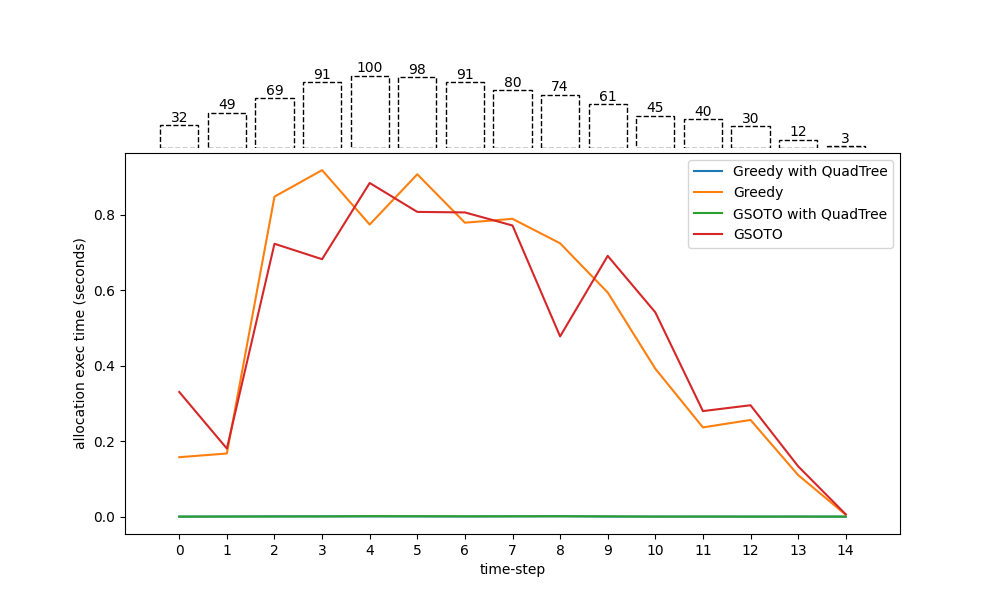
\includegraphics[width=.7\linewidth]{images/graphs/exec_QT_prov.png}
    \caption{Auction execution times with and without the use of Quad Tree data structure, with the number of users on each time-step.}
    \label{fig:exec_qt}
\end{figure}
The chart shows that the Greedy and GSOTO using the data structure were very much faster than the algorithms not using it. Even in the time-steps with small number of users, like at the beggining of the simulation, they  took almost $0.2$ seconds, while the others using QuadTree kept in the same scale during the entire simulation, even with $100$ users in time-step $5$.

This occurs because, for each user $\user \in \setofUsers$,  the algorithms without the QuatTree iterate on every cloudlet in the system until find the one that fits the user and does not violate their latency constraint. On other hand, the algorithms using the QuadTree can filter only the cloudlets in a reasonable distance of the users, which decreases the number of iterations significantly.

Because of this improvement, in the following subsections we consider only the Greedy and GSOTO using Quadtree to analyse the results.

\subsection{Execution times}
The auction execution time is an important metric to be analyzed because it is directly related to the scalability of the auction mechanism. We analyze it in Fig.~\ref{fig:time}, where in Fig.~\ref{fig:alloc_exec} we have the execution time of the allocation step of the auctions, and in Fig.~\ref{fig:auction_exec} we have the total time of the auctions, which is the sum of the allocation and pricing steps. In both charts, we have the number of users in the system on each time-step represented as bars on the top of the chart.
\begin{figure}[H]
    \centering
    \begin{subfigure}{.45\textwidth}
        \centering
        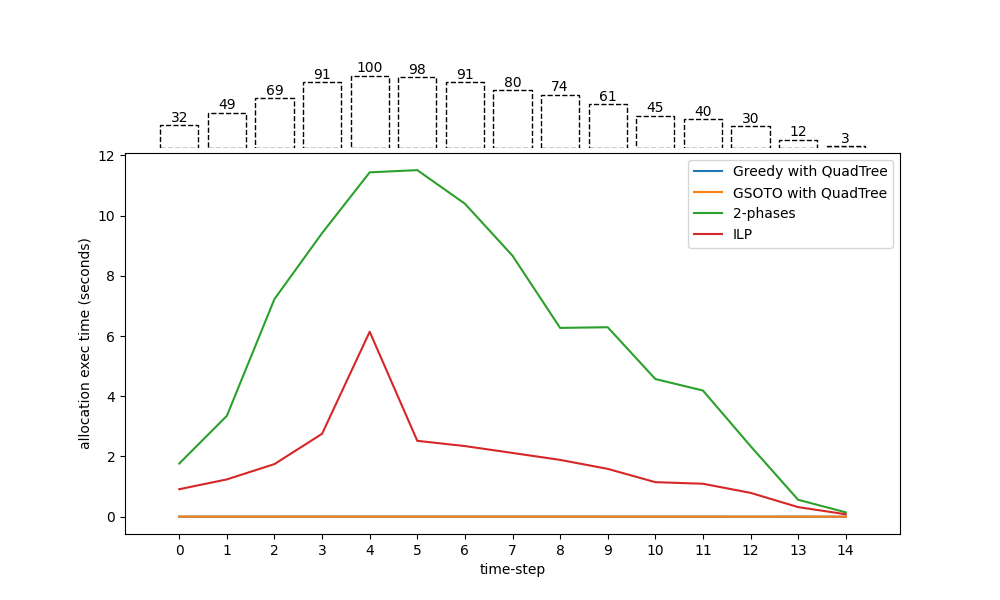
\includegraphics[width=.9\linewidth]{images/graphs/alloc_exec.png}
        \caption{Allocation execution time, with the number of users represented  on each time-step.}
        \label{fig:alloc_exec}
    \end{subfigure}
    \begin{subfigure}{.45\textwidth}
        \centering
        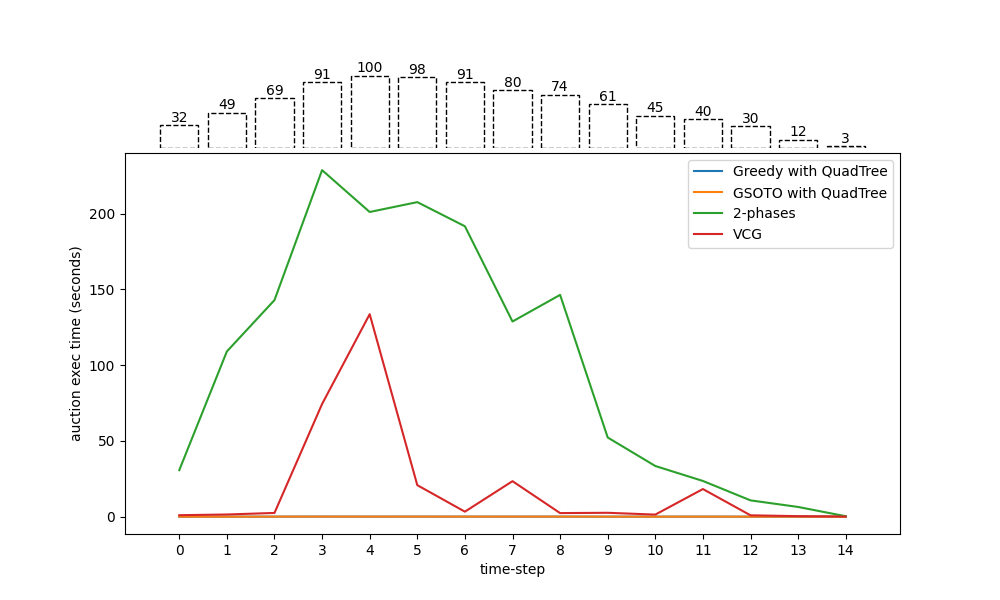
\includegraphics[width=.9\linewidth]{images/graphs/auction_exec.png}
        \caption{Auction (allocation + pricing) execution time, with represented the number of users on each time-step.}
        \label{fig:auction_exec}
    \end{subfigure}
    \caption{Execution times of the auction approaches.}
    \label{fig:time}
\end{figure}
In Fig.~\ref{fig:alloc_exec}, we notice that the 2-phases takes more time to finish the allocation step than the other algorithms. This slower execution is mainly caused by the second phase of this algorithm where we have to execute a Maximum Flow algorithm to find the maximum matching between the users and the cloudlets.

The ILP approach was better than the 2-phases but still took more time than the other two allocation algorithms. This is because the ILP approach has to solve a linear program to find the allocation, which can be very costly depending on the number of users and cloudlets in the system, as we can seen the execution time with 100 users in time-step $4$.  

The Greedy and GSOTO were in the same scale of execution time, and they were the fastest algorithms. This is because they are greedy approaches, which means that they do not have to solve any complex problem to find the allocation, they just have to iterate on the users and cloudlets to find the best allocation for each user. Even better because of the use of the QuadTree, as we said in the previous subsection.

By looking at the auction execution times in Fig.~\ref{fig:auction_exec}, we can see the how complex is to execute the pricing step using the VCG-based pricing. This is because, for each winner, we have to simulate an allocation without him to find the price. This is the reason why the VCG-based pricing took more time than the critical pricing, which can be also costly, but it just have to find the maximum bid of the users that can be allocated without the winner by iterating on the users and cloudlets. This is more clear in time-step $4$, where the VCG-based pricing took almost $120$ seconds to finish the auction, while the critical pricing used in the others took less than $10$ seconds.

As we saw in the allocation step, the two-phases took more time than the other algorithms, and this is also true for the auction execution time. However, the pricing step of the 2-phases is relatively fast because only the winners from the first phase has prices to be calculated. So, this auction execution time of it is mainly caused by the allocation step.

Finally, the auction execution time of the Greedy and GSOTO, we notice again that they were in the same scale of execution time, and they were the fastest algorithms. They are very similar in execution time because the basically use the same greedy approach in the auction, where the only difference is the criteria to sort the users, where the GSOTO uses the ratio between the user's bid and the sum of their requirements, while the Greedy uses the ratio between the user's bid and only the maximum requirement of the user instead of the sum of it.


\subsection{Social welfare and prices}
We analyse the social welfare achieved by each approach by plotting a chart with the cumulative value of them on each time-step, as we can see in Fig.~\ref{fig:sw}. We also plot the cumulative profit achieved by the cloudlets in Fig.~\ref{fig:profit}. TO better understand this both charts, we also plot the number of winners on each time-step in Fig.~\ref{fig:winners}, and the distribution of them during the entire simulation in Fig.~\ref{fig:winners_dist}.

The VCG has the best result in terms of social welfare, which is expected because it calculates and optimal allocation that maximizes the social welfare. However, it is not the best in terms of profit and number of winners.

The Greedy and GSOTO has similar results, and they are very close to the VCG in terms of social welfare, which show that it can maximize the social welfare and achieve results close to an optimal. However, GSOTO were slightly better than Greedy, showing that the ratio between the user's bid and the sum of their requirements can be better criteria to sort the users than the ratio between the user's bid and only the maximum requirement of the user instead of the sum of it.

The GSOTO is also better in terms of profit and number of winners. It has more winners than the Greedy, which means that it can allocate more users than the Greedy, and also has more profit than the Greedy, which leads to the allocation of the users with the most profitable bids.

The 2-phases has the worst result in terms of social welfare, compared to the others. This is primarily caused by two factors: this approach does not allocate as much users as the others, which is afact that we can see in Fig.~ref{fig:winners_dist}, and also because it does not chose the users with the most profitable bids, which means that it does not maximize the social welfare efficiently.

However, the 2-phases has the best result in terms of profit, which is expected because it allocates the users with the most profitable bids, as we can see in Fig.~\ref{fig:profit}. This is also the reason why it has the least number of winners, because it allocates the users with the most profitable bids, which means that it does not allocate the users with the least profitable bids, as we can see in Fig.~\ref{fig:winners_dist}.
\begin{figure}
    \centering
    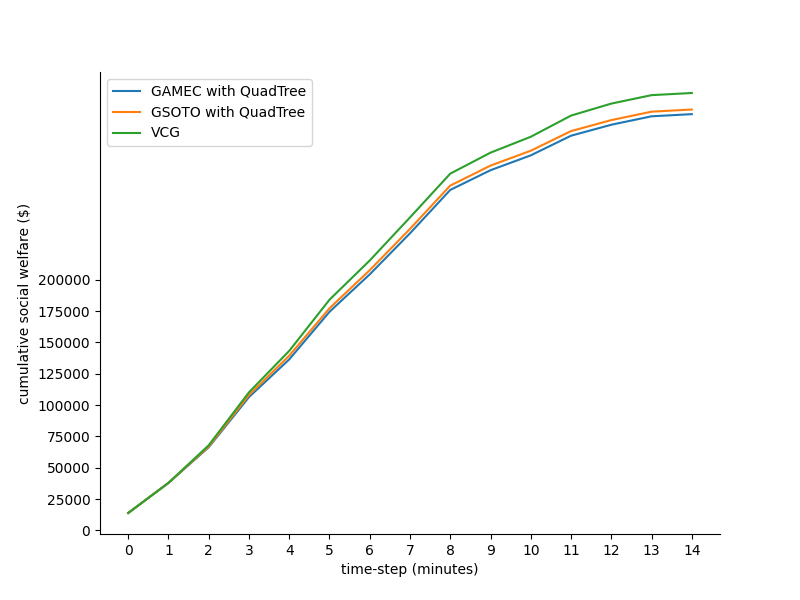
\includegraphics[width=.7\linewidth]{images/graphs/sw.png}
    \caption{Cumulative social welfare achieved.}
    \label{fig:sw}
\end{figure}

\begin{figure}
    \centering
    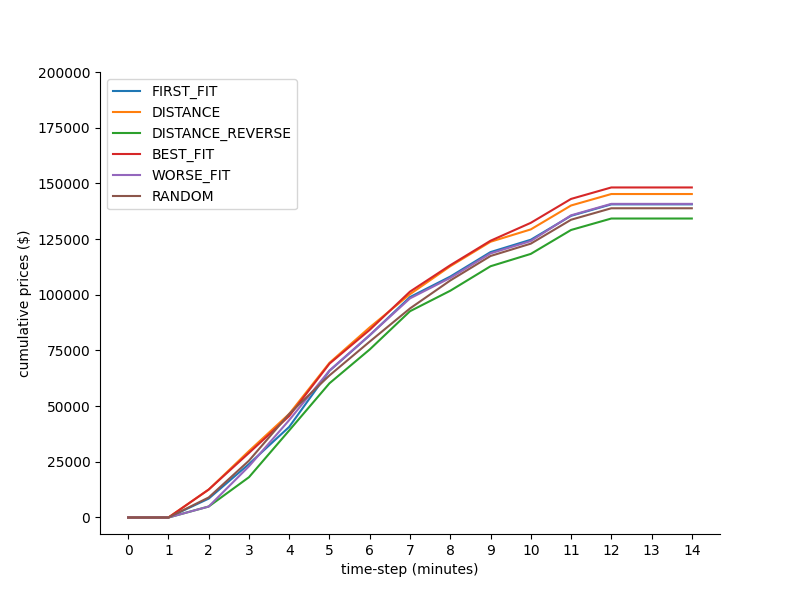
\includegraphics[width=.7\linewidth]{images/graphs/prices.png}
    \caption{Cumulative profit achieved.}
    \label{fig:profit}
\end{figure}

\begin{figure}
    \centering
    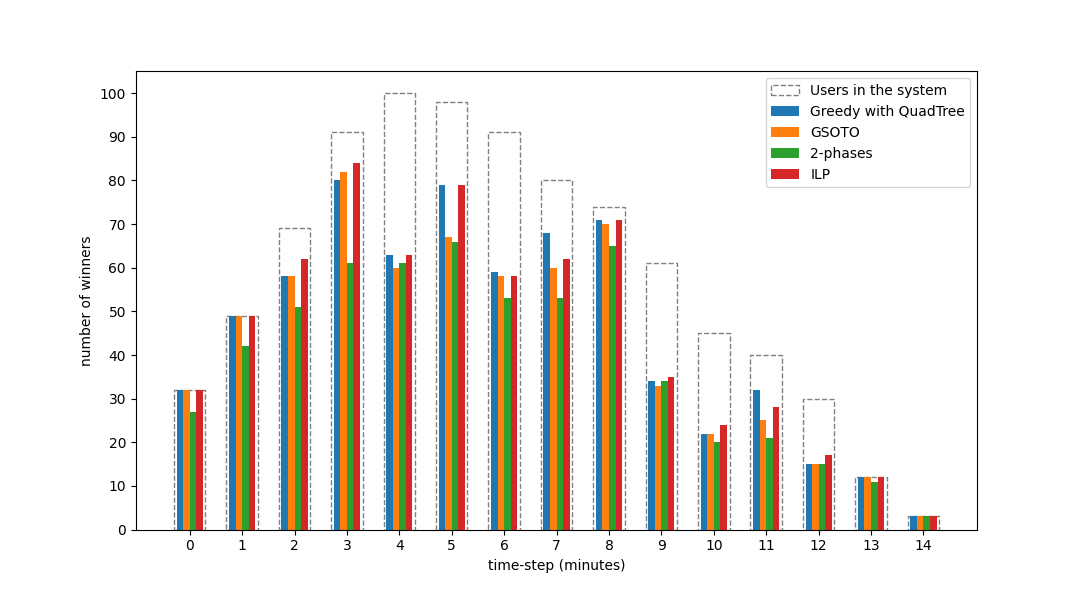
\includegraphics[width=.7\linewidth]{images/graphs/winners_bars.png}
    \caption{Number of winners on each time-step.}
    \label{fig:winners}
\end{figure}

\begin{figure}
    \centering
    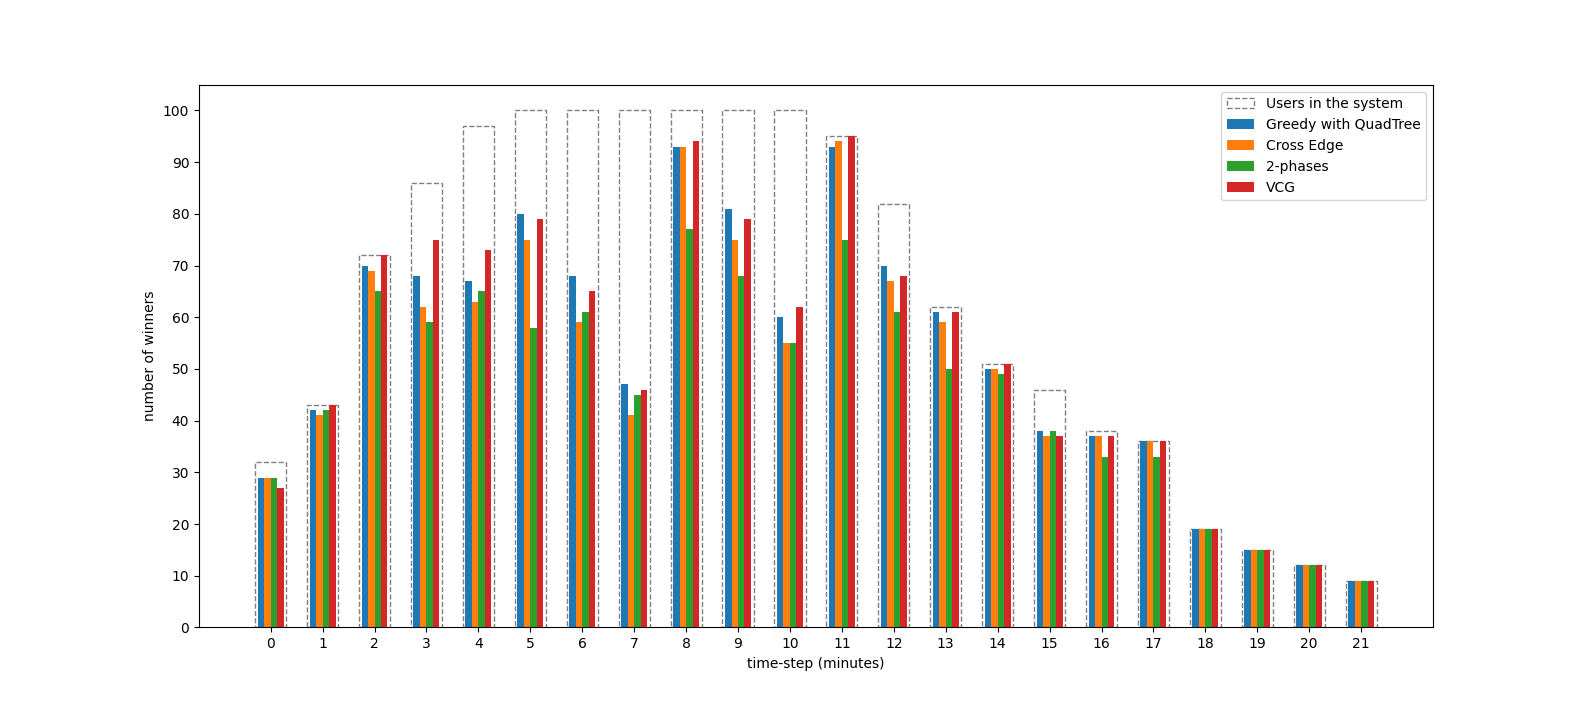
\includegraphics[width=.7\linewidth]{images/graphs/winners_bp.png}
    \caption{Distribution of winners.}
    \label{fig:winners_dist}
\end{figure}

\subsection{Latency}
The latency of the users is an important metric to be analysed because it is directly related to the quality of the service provided by the cloudlets. Also, it is very related to the mobility of the users, because the users that are moving faster will have higher latencies than the users that are moving slower. So, we analyse the latency of the users by plotting a bioxplot chart where we have a boxplot for each of the approaches, as we can see in Fig.~\ref{fig:lat}.
\begin{figure}
    \centering
    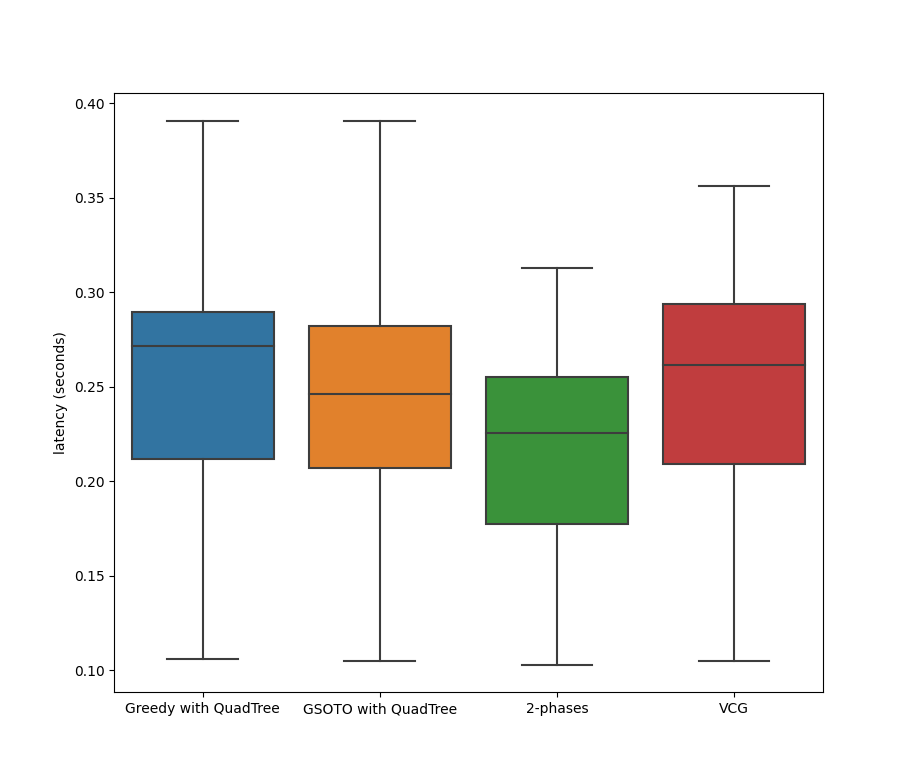
\includegraphics[width=.7\linewidth]{images/graphs/lat_bp.png}
    \caption{Distribution of latency of the users.}
    \label{fig:lat}
\end{figure}

We can see that the 2-phasese has the best result in terms of latency, and this is related to the way this approach calculates the allocation. In the first phase, each cloudlet detects the users inside their coverage radius, taking the users very close to them. And in the second phase, to calculate the maximum flow, the arcs from the users to the cloudlets vertices are weighted by the latency of the users, which means that the users with the lowest latency will have the highest flow, and the users with the highest latency will have the lowest flow. So, the users with the lowest latency will be allocated to the cloudlets, and the users with the highest latency will not be allocated. This is the reason why the 2-phases has the best result in terms of latency.

\subsection{Cloudlets resource usages}
We analyse the resource usages of the cloudlets by plotting a chart with the CPU, RAM and storage used on each time-step, as we can see in Fig.~\ref{fig:cpu}, Fig.~\ref{fig:ram} and Fig.~\ref{fig:storage}, respectively. The idea is to verify if the auction approaches are able to allocate the users in a way that the cloudlets are better used.
\begin{figure}
    \centering
    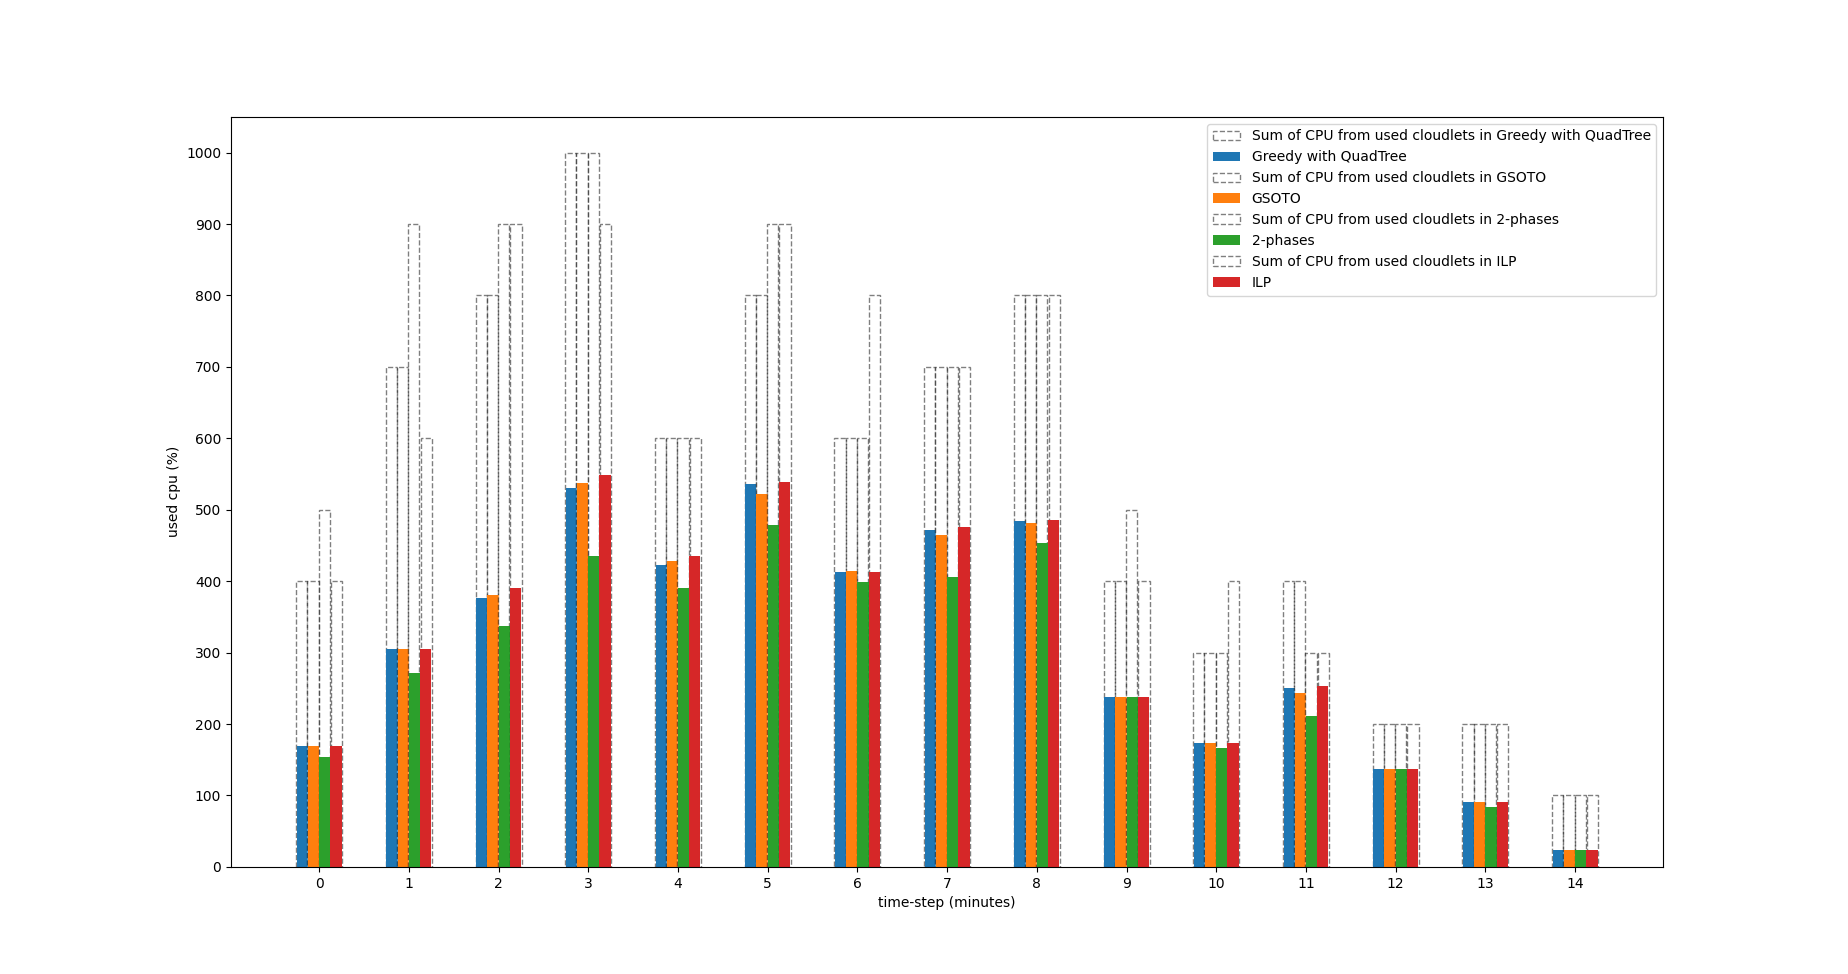
\includegraphics[width=.7\linewidth]{images/graphs/res/cpu.png}
    \caption{CPU usage on each time-step.}
    \label{fig:cpu}
\end{figure}
The results of CPU used in the cloudlets are similar for all the approaches. The cloudlets are not used in a way that they are always close to 100\% of usage at none of the time-steps. It can happen because the CPU was not the most decision factor in most of the cases of allocation. For example, there might be a case where the VM to be allocated is RAM-intensive, but the cloudlet has a lot of CPU available, so it can allocate the VM, even if the CPU is not the most important resource for the VM.
\begin{figure}
    \centering
    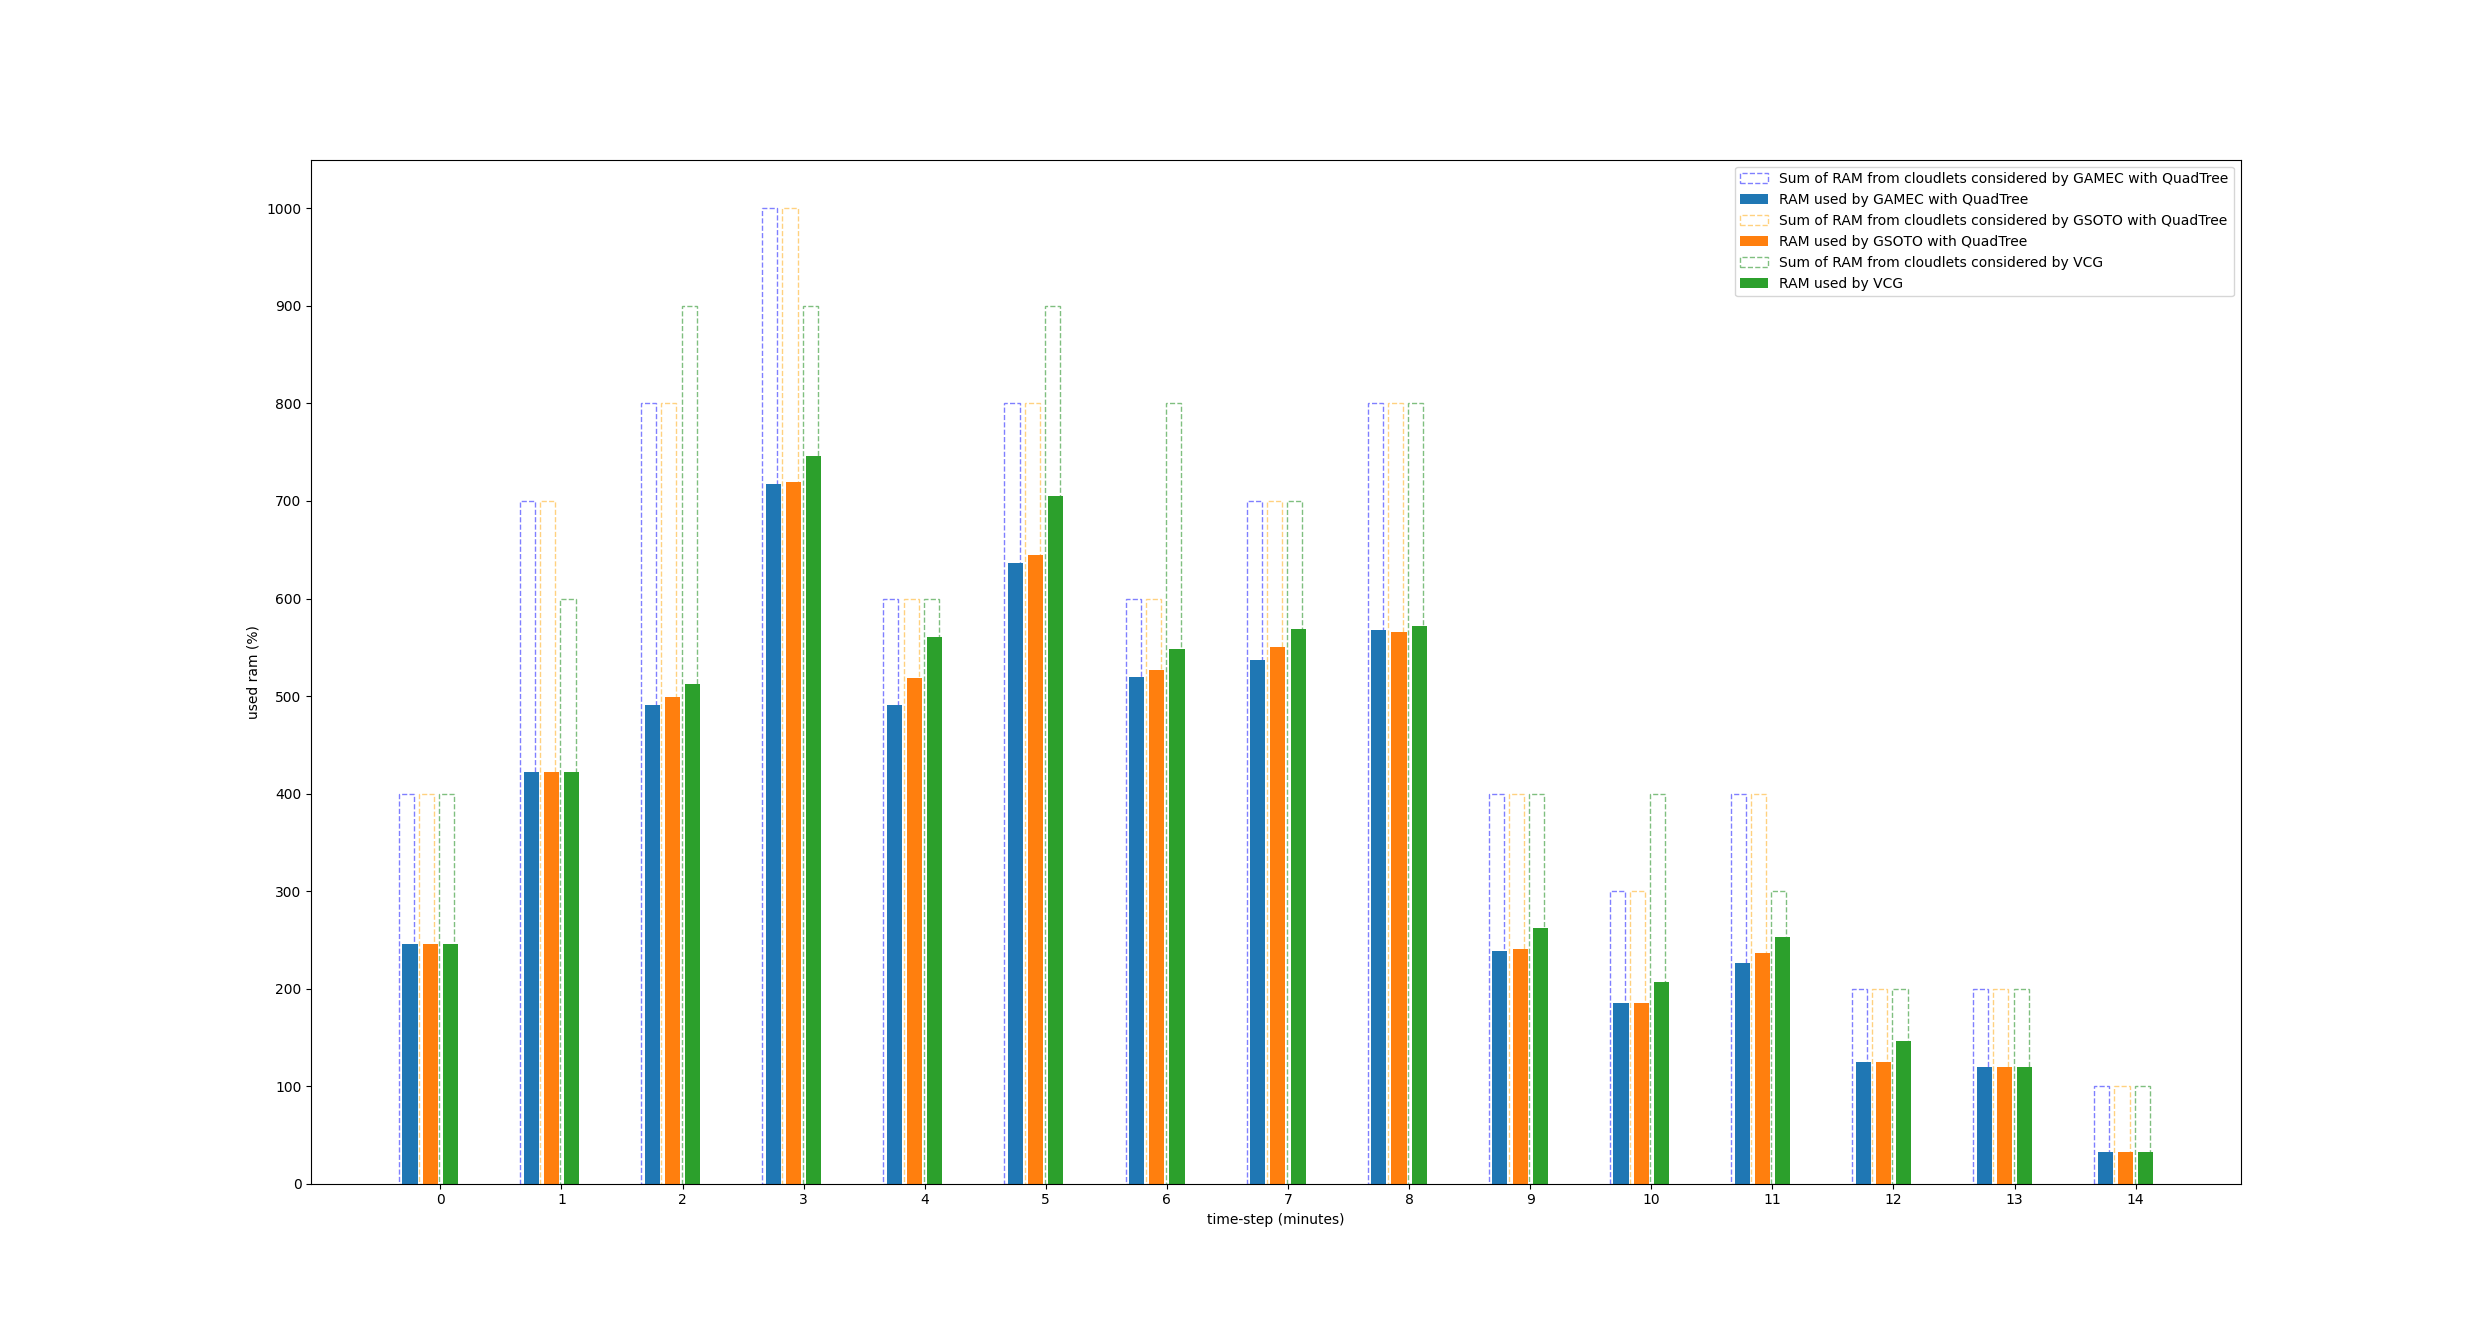
\includegraphics[width=.7\linewidth]{images/graphs/res/ram.png}
    \caption{RAM used on each time-step.}
    \label{fig:ram}
\end{figure}
The use of RAM better used than the CPU. It is related to the VMs' parameters as defined in Section~\ref{sec:sim_parameters}, because the RAM values from different VMs are quite discrepant, even more in the VM type c6gn.2xlarge, also defined as RAM-intensive. So, the cloudlets are better used in terms of RAM than in terms of CPU.

\begin{figure}
    \centering
    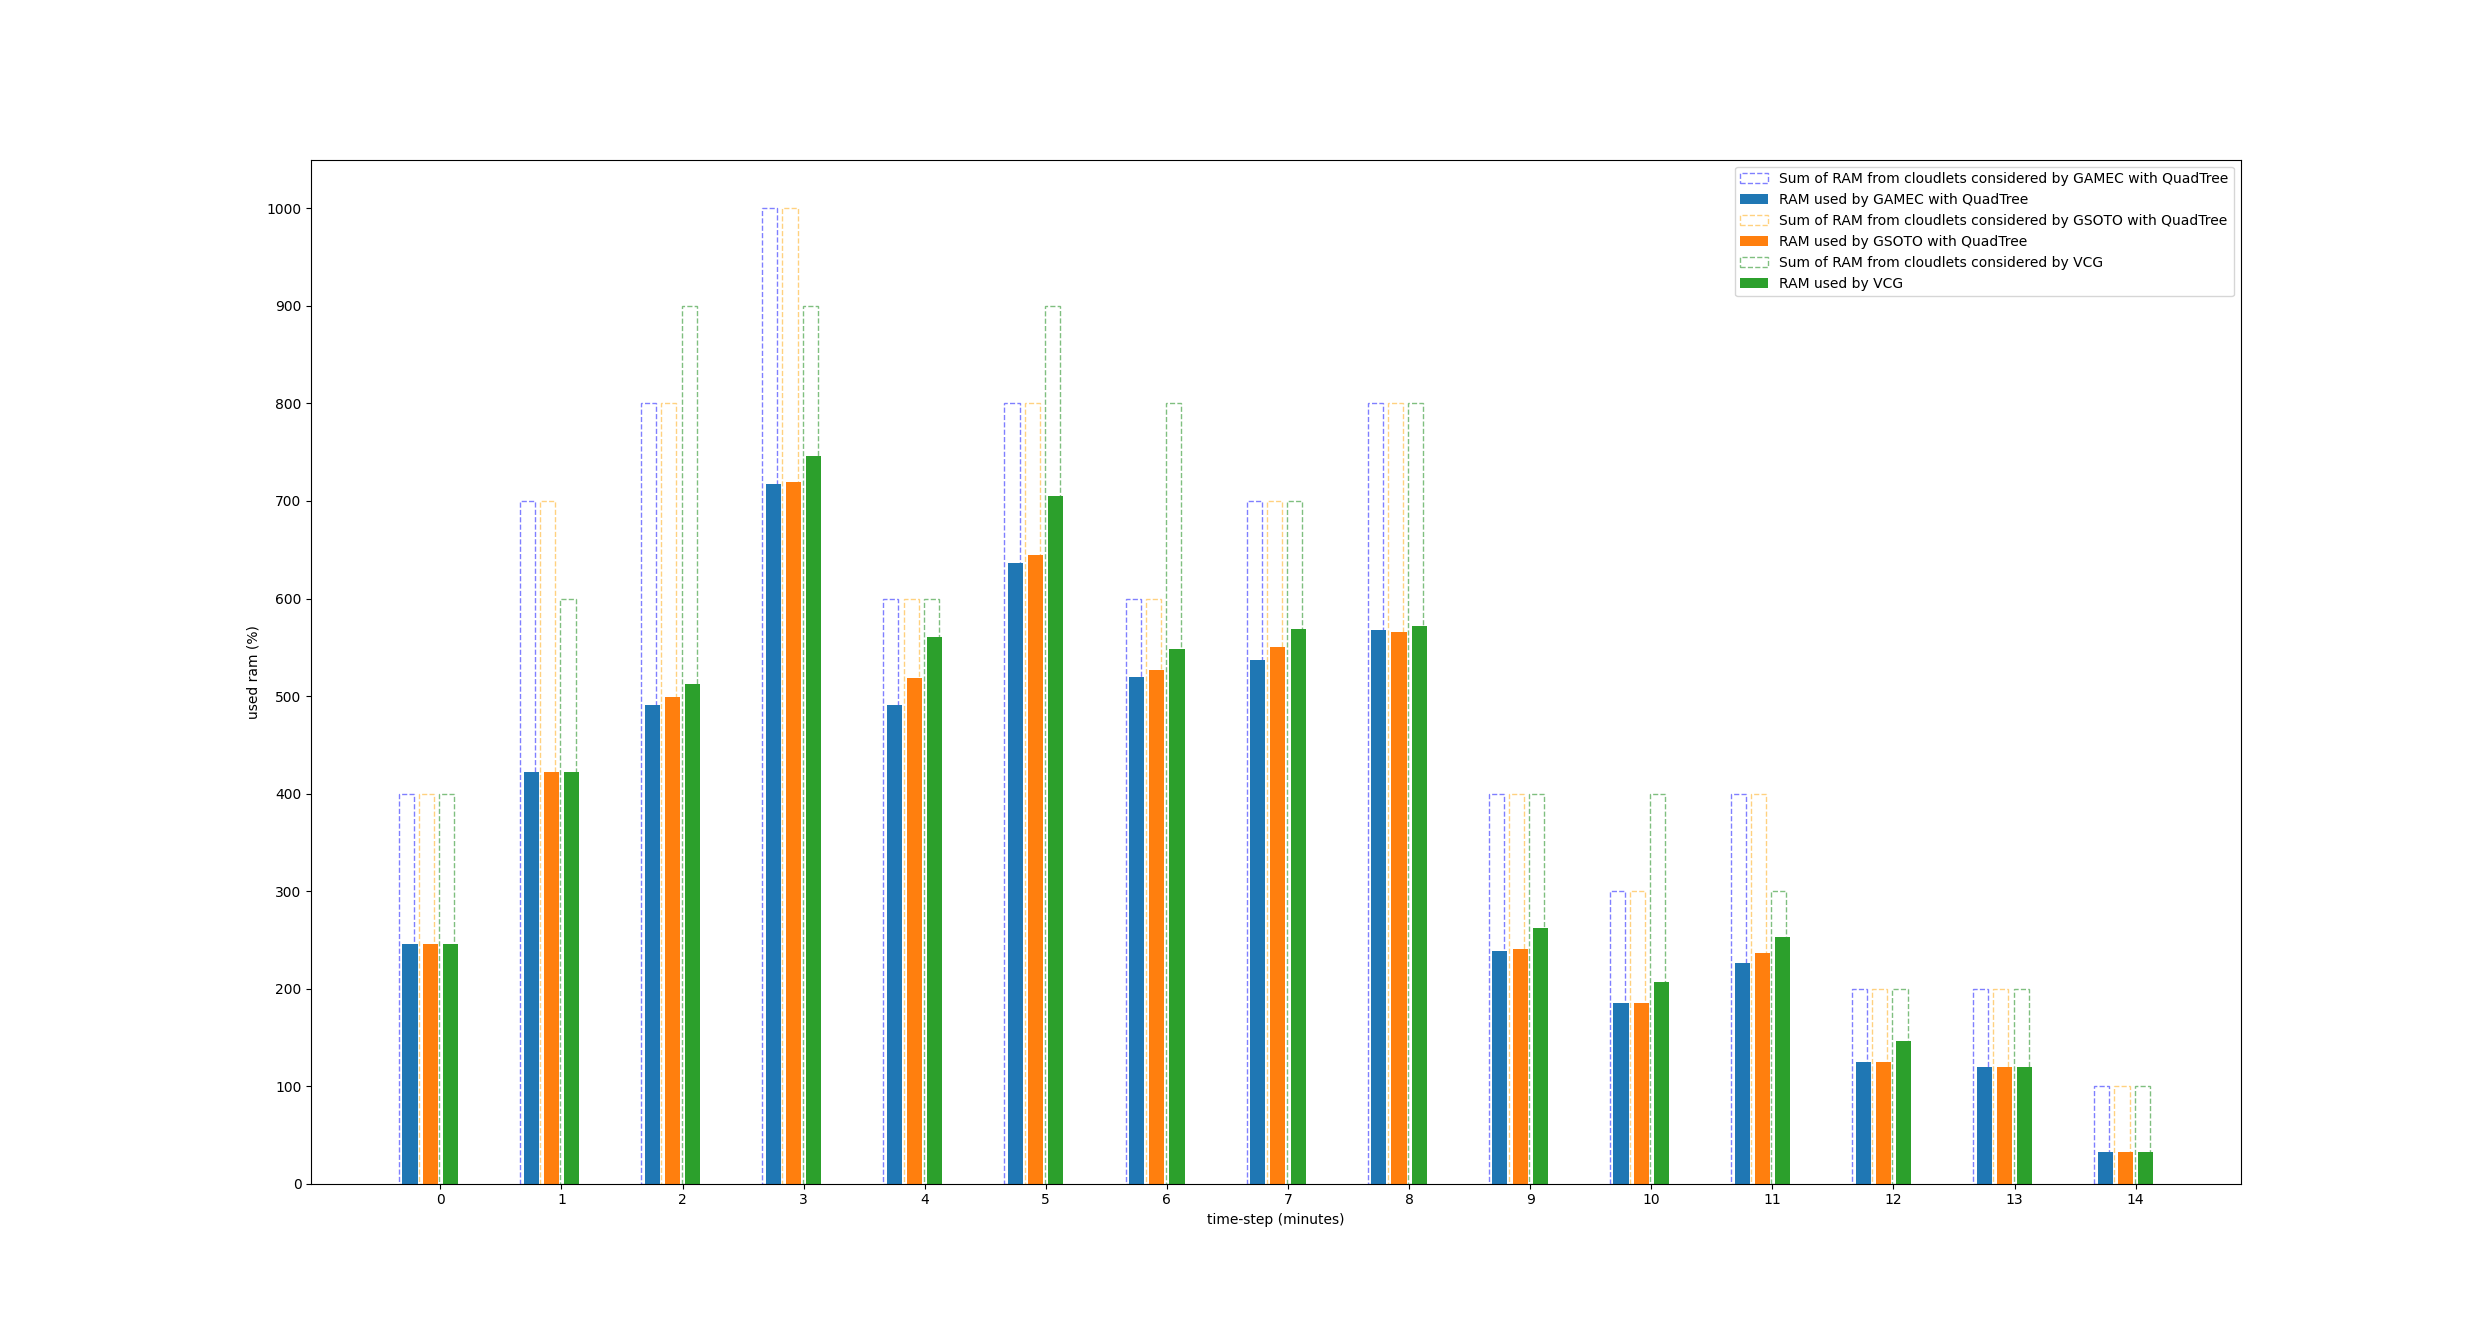
\includegraphics[width=.7\linewidth]{images/graphs/res/ram.png}
    \caption{Storage used on each time-step.}
    \label{fig:storage}
\end{figure}
The storage of the cloudlets are similar to the RAM, but here we have a case where the ILP used almost the total amount of available resource, as we can see in time-step $11$.

\chapter{Conclusions}
\label{ch:conc}
In this work, we propose two greedy-based auction mechanisms for the allocation problem in Edge Computing environments: the Greedy and the 2-Phases.

The first one is based on the idea that the allocation problem with multiple cloudlets offering resources and multiple users requesting for these resources can be seen as a MMKP problem, then we use a greedy approach where the users are sorted by the ratio between their bids and the maximum of their requirements and try to allocate them in the available cloudlets, according to the defined constraints. Then, we use a critical pricing-based approach to define the prices for the users that were allocated, ensirung truthfulness and individual rationality.

The second one is divided in two parts. In the first, each cloudlet in the system detects the user inside its coverage radius and execute a greedy algorithm for them, similar to the greedy from the latter auction, but here it is modeled as a MKP problem, i.e., only one cloudlet for multiple users. After this, in the second phase, we take separete the users allocated and unallcoated in the first phase and execute a Maximum Flow algorithm, enabling the unallocated users to be allocated in other cloudlets, if possible. Then, we also use a critical pricing-based approach to define the prices for the users allocated in the first phase, and the prices for the users allocated in the second phase are defined as zero, because their bids were not used in the allocation.

We also modeled a VCG-based auction mechanism for this same allocation problem, where we have an ILP model that defines the allocation and the Clarke Pivot Rule defines the prices of the winners.

For the experiments, we used a real dataset from the Interscity project, which contains the bus lines and the cloudlets in the city of Sao Paulo - Brazil. We also used a simulator to execute the experiments, where we defined the parameters of the cloudlets and the users, and then we executed the auctions for the users in the system. We also implemented an auction mechanism from the literature to compare with our mechanisms.

We see that the Quad Tree data structure was very useful to improve the execution time of the first greedy auction mechanism and also the adapted auction from the literature, GSOTO.

Also, the results show that our mechanisms have a better performance than the VCG-based auction, in terms of execution time, mainly when we consider the time on the entire auction, because the VCG needs to execute an optimization for every winner, and it is very costly.

When we look at the 2-phases results, we see that it takes more time to execute each auction, even more in the second phase, responsible to execute a Maximum Flow algorithm. However, the latency of the users allocated by this approach has lower values in the experiments.

Finally, we see that the GSOTO auction has a better execution time than the two greedy approaches we modeled, and it shows us that the sorting method used by~\cite{WeifengAuction2022} using the sum of the requirements of the users can better than the maximum of the requirements, as we used in our greedy approaches.

For future works, we can improve the 2-phases auction mechanism by using a better algorithm to allocate the users in the second phase, instead of the Maximum Flow, which is a very costly algorithm. We can also improve the Greedy-based auction by using a better sorting method, like the one used by GSOTO, and also by using a better pricing method, instead of the critical pricing, which is not very good in terms of social welfare and prices. Besides, another direction can be to improve the auction mechanisms for Edge Computing with prediction methods, where the Edge COmputing system can predict the users' requirements and bids, and then use this information to improve the allocation and pricing of the users.

% As referências:
\bibliographystyle{plain}
\bibliography{references/ic-tese-v3}


% Os anexos, se houver, vêm depois das referências:
% \appendix
% \chapter{Anexo 1}
% \chapter{Anexo 2}

\end{document}
